\documentclass[a4paper, 12pt]{article}
\usepackage{fontspec}
%\usepackage[utf8]{inputenc}
\usepackage{graphicx}
\usepackage{float}
\usepackage{hyperref}
\usepackage[margin=2cm]{geometry}
\usepackage{amsmath}
\usepackage[nottoc,numbib]{tocbibind}
\usepackage{enumerate}
\usepackage{indentfirst}
\usepackage{algorithm}
\usepackage{algpseudocode}
\usepackage{amssymb,latexsym,stmaryrd,dsfont,amsthm, algorithmicx}
\usepackage[polish]{babel}
%\usepackage{polski}

\newcommand{\image}[2]{
\begin{center}
\includegraphics[scale = #1]{#2}
\end{center}
}

\newcommand{\capimage}[3]{
\begin{center}
\includegraphics[scale = #1]{#2}\\
\small #3 \normalsize
\end{center}
}

\title{\textbf{Symulacja ruchu ludzi w centrum handlowym}}
\author{Paweł Kłeczek \\ \emph{pkleczek@student.agh.edu.pl} \and Kajetan Rzepecki \\ \emph{kajetan.rzepecki+agh@gmail.com}}
\date{\today}

\begin{document}

    \maketitle

    \vfill
    \begin{abstract}
    % TODO Trzeba dodać coś więcej IMO, na przykład o tym, jak podejdziemy do problemu ruchu ludzi.

\noindent
Praca i związany z nią projekt dotyczą symulowania ruchu ludzi w centrum handlowym z wykorzystaniem modelu \emph{Social Distances} na dwuwymiarowej siatce.
    \end{abstract}
    \vfill

    \thispagestyle{empty} % Nie chcemy numerować pierwszej strony.

\newpage
    \setcounter{page}{1}
    \setcounter{tocdepth}{3}

    \tableofcontents

\newpage
    \section{Wprowadzenie}
    \label{sec:intro}

\noindent
Celem wykonywanego projektu jest stworzenie modelu oraz symulacja ruchu ludzi w centrum handlowym w oparciu między innymi o model \emph{Social Distances} (\cite{refs:social-distances-1, refs:social-distances-2}).

Modelowanie ruchu dużych grup ludzi w środowisku centrum handlowego jest problemem złożonym i wymaga wykorzystania równie złożonych algorytmów celem dokładnego przybliżenia rzeczywistych zachowań. Dobrym podejściem jest dekompozycja problemu modelowania złożonego zjawiska na mniejsze, łatwiejsze do rozwiązania podproblemy, którymi zajmują się osobne, dobrze zdefiniowane i wyspecjalizowane algorytmy, i ponowne połączenie wyników ich działania w spójną całość - metoda \emph{Divide and Conquer}.

    \begin{figure}[H]
        \centering
        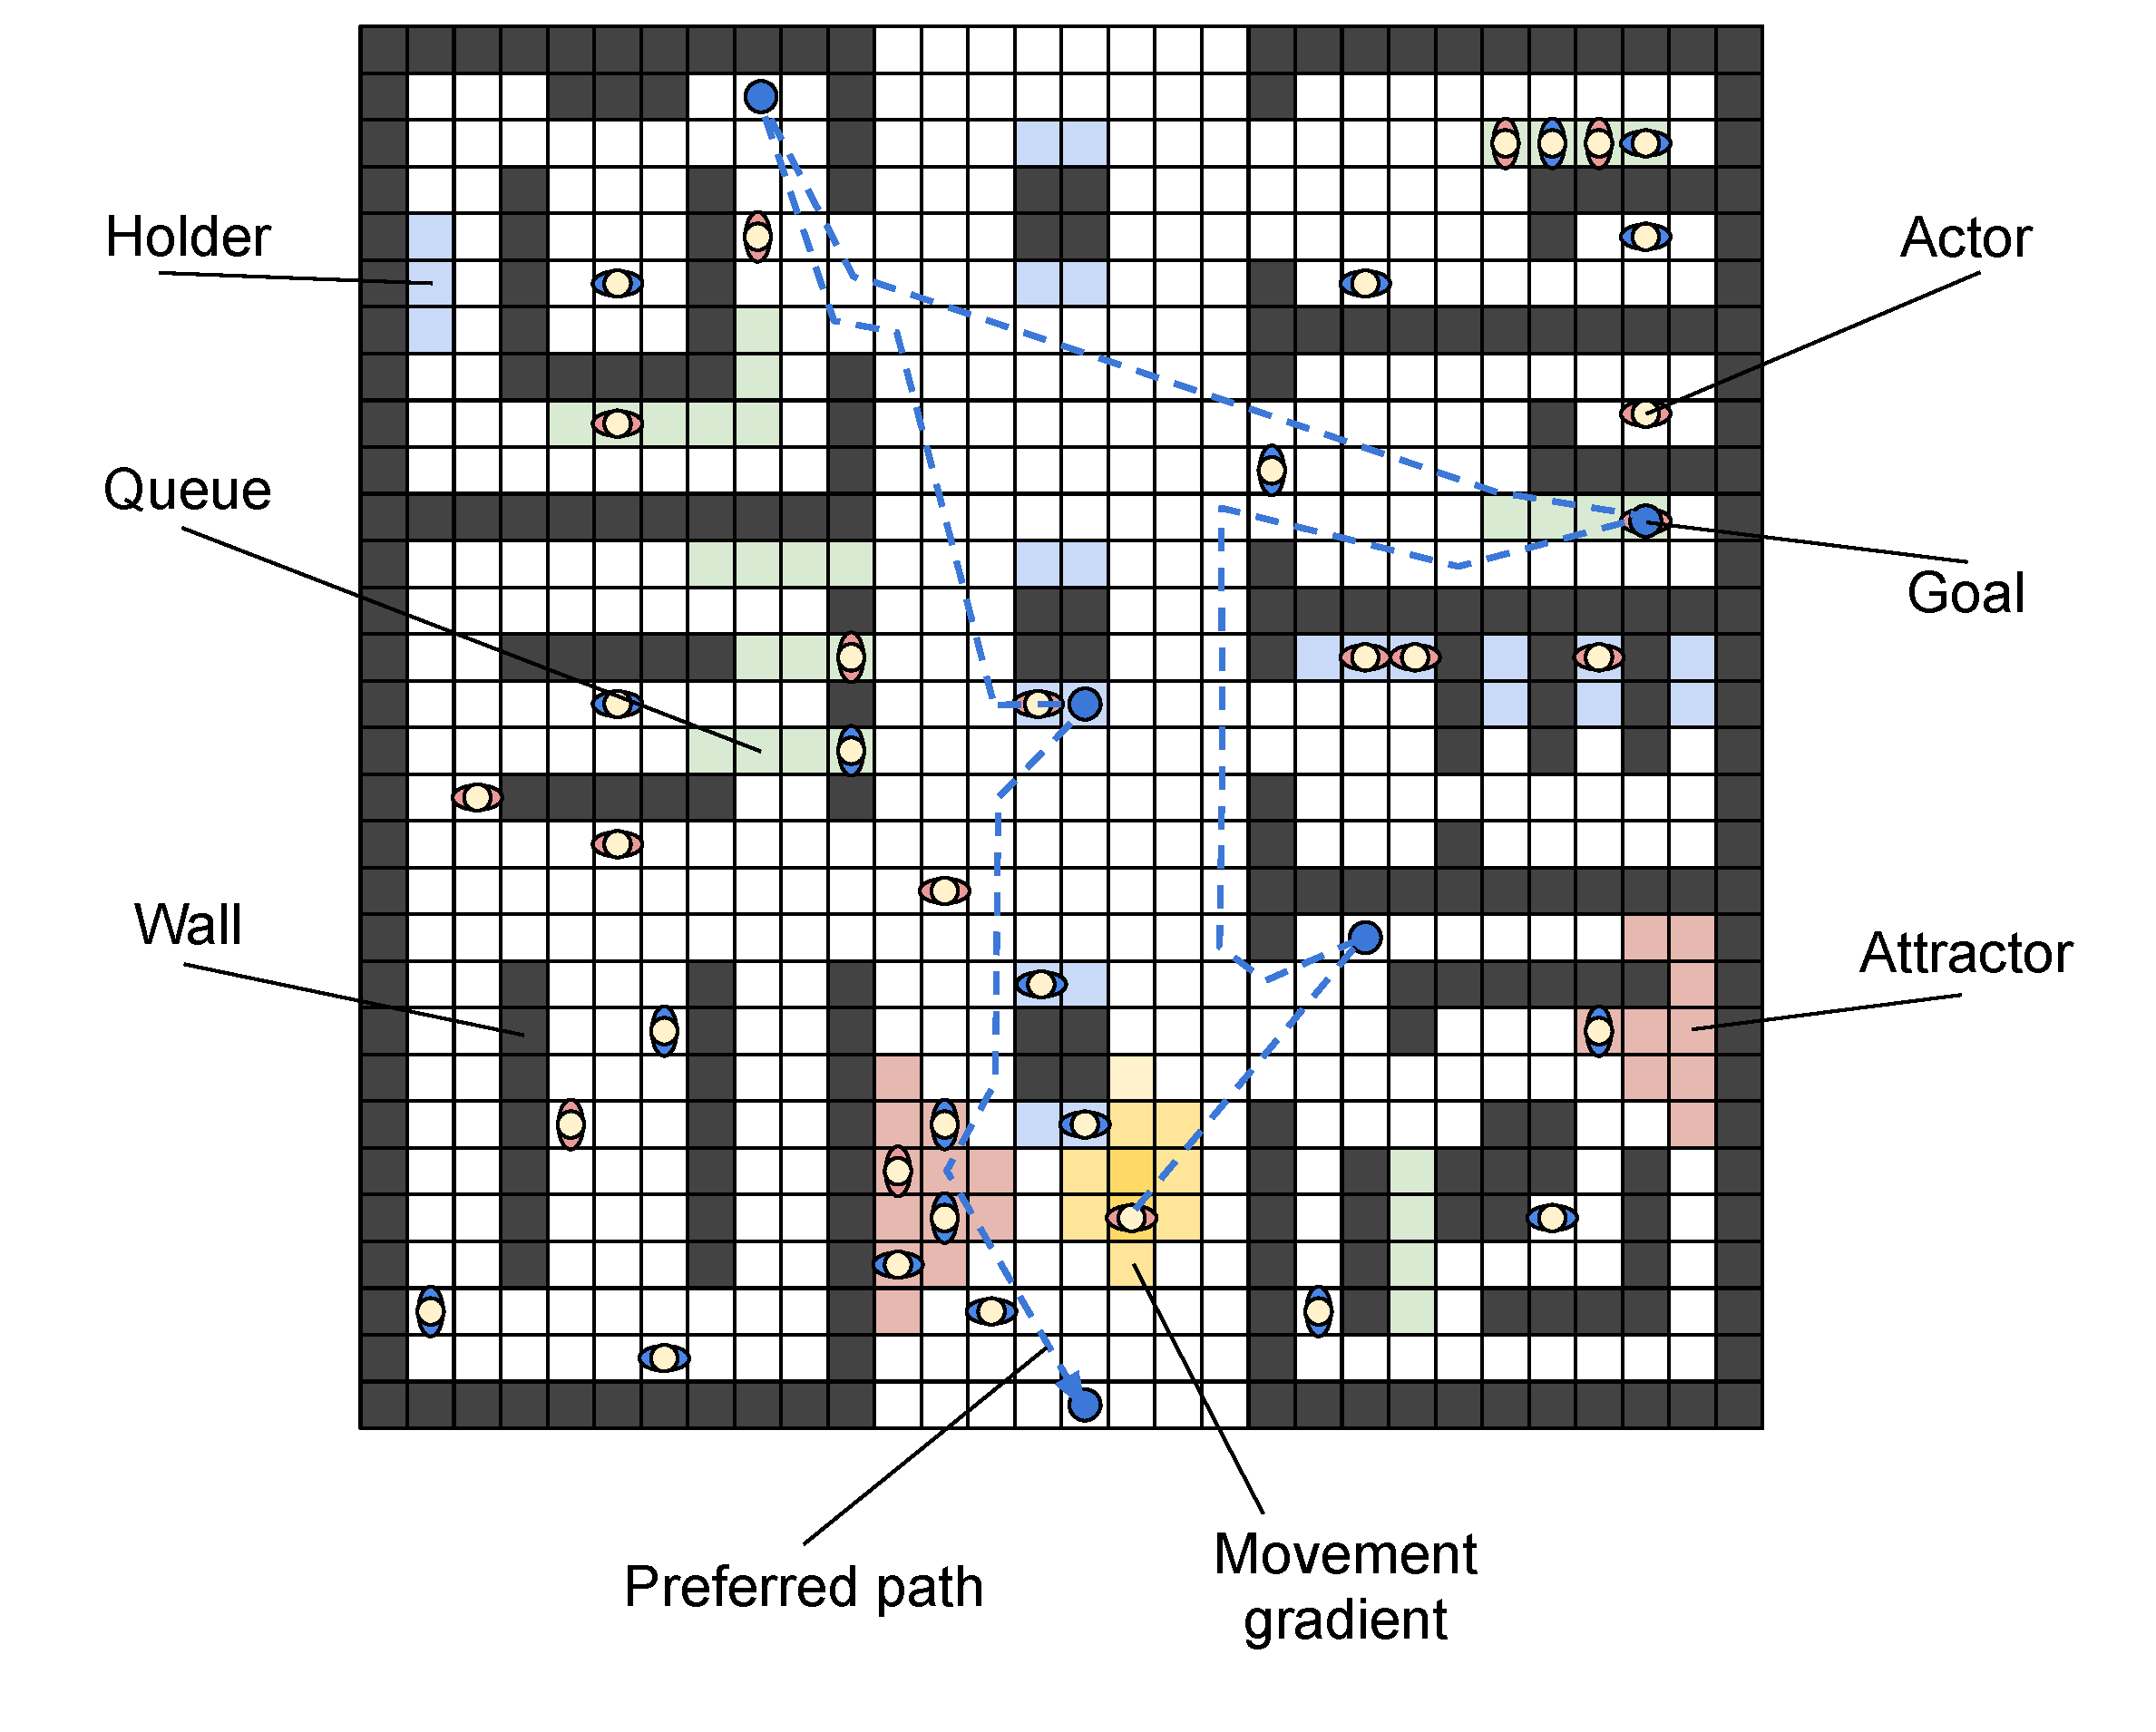
\includegraphics[scale=0.3]{./img/Overview.pdf}
        \caption{Przykładowa dekompozycja problemu modelowania ruchu ludzi w centrum handlowym.}
        \label{fig:decomp}
    \end{figure}

W zależności od domeny rozwiązywanego problemu dekompozycja może zachodzić ze względu na wiele czynników i dotyczyć różnych aspektów problemu - np. podział wejściowego zbioru danych na dwa mniejsze podzbiory w algorytmie \emph{Quick sort}, czy podział modelu ruchu ludzi na elementarne zachowania, jak \emph{kolejkowanie}, \emph{atrakcja} lub \emph{oczekiwanie}.

Na rysunku \ref{fig:decomp} została przedstawiona przykładowa dekompozycja problemu poruszanego w tym dokumencie. Wyszczególniono w niej podział na globalną, preferowaną ścieżkę wiodącą poruszającego się po centrum handlowym agenta do obranych przez niego celów i lokalny ruch zgodny z gradientem ruchu obliczonym na podstawie jego otoczenia. Dodatkowo zastosowano podział na specjalne strefy odpowiedzialne za modelowanie elementarnych zachowań ludzi w centrach handlowych, takie jak strefy kolejek, czekania i gromadzenia się, które realizowane są za pomocą innych modeli ruchu.

\newpage
    \subsection{State of the art}
    \label{sec:sota}

\noindent
Zagadnienia modelowania ruchu ludzi są od długiego czasu postrzegane jako istotne z punktu widzenia usługowego. Już w latach 80 ubiegłego wieku Aloys Borgers i Harry Timmermans zajmowali się modelowaniem ruchu pieszych w środowisku centrum handlowego w oparciu o modele probabilistyczne (\cite{refs:route-choice-1}).
Na przestrzeni lat modele ruchu pieszych ewoluowały w wielu kierunkach, od dynamiki płnów (\cite{refs:fluid-dynamics}) przez automaty komórkowe (\cite{refs:cellular-movement}) i algorytmy genetyczne (\cite{refs:pedestrian-behaviour-2}) aż do modeli opartych o systemy wieloagentowe (\cite{refs:real-data-2}). \\

\emph{Cellular automata microsimulation for modeling bi-directional pedestrian walkways} \linebreak (\cite{refs:cellular-movement}) skupia się na modelowaniu dwukierunkowego ruchu ludzi z wykorzystaniem automatów komórkowych. Praca ta dowodzi, że stosunkowo nieskomplikowany automat komórkowy z małą liczbą reguł jest zdolny do symulowania skomplikowanych zachowań, które dobrze oddają rzeczywistość. Zaproponowany model i algorytm \textbf{CA-ped} pozwalają symulować ruch ludzi w dwóch przeciwnych kierunkach na dwóch oddzielnych jak i mieszanych pasach ruchu, a także dynamicznych, wieloliniowych (\emph{dynamic multi-lane, DML}) pasach ruchu.

Algorytm \textbf{CA-ped} wyróżnia dwie fazy ruchu, z których każda charakteryzuje się trzema prostymi zasadami:

\begin{enumerate}
    \item Zmiana pasa ruchu
        \begin{itemize}
            \item Eliminacja konfliktów - dwóch przechodniów nie może znajdować się na jednej komórce, w przypadku konfliktu wolna komórka oddzielająca dwóch przechodniów jest przyznawana jednemu z nich z równym prawdopodobieństwiem.
            \item Identyfikacja wolnych przestrzeni - wybierany jest ten pas ruchu, który cechuje największa liczba wolnych komórek, co implikuje bezproblemowy ruch w przyszłości.
            \item Zmiana pasa - każdy przechodzień jest poruszany na jeden z dwóch sąsiednich pasów, lub pozostaje na obecnym pasie ruchu.
        \end{itemize}
    \item Ruch do przodu
        \begin{itemize}
          \item Obliczanie szybkości ruchu - dla każdego przechodnia obliczana jest jego szybkość uzależniona od istnienia, bądź nie, wolnych komórek w jego otoczeniu.
          \item Wymijanie - jeśli bezpośrednio przed przechodniem w niedużej odległości istnieje przeciwstawny przechodzień, to z zadanym prawdopodobieństwiem następuje wyminięcie obu przechodniów.
          \item Ruch - każdy przechodzień jest przemieszczany do przodu zgodnie z szybkością jego ruchu.
        \end{itemize}
\end{enumerate}

\emph{Pedestrian behaviour modelling - An application to Retail Movements using a Genetic Algorithm} (\cite{refs:pedestrian-behaviour-2}) identifikuje problemy i nieścisłości wynikające ze stosowania modeli opartych o najkrótsze ścieżki (\emph{shortest-paths}) i maksymalizację przydatności (\emph{utility-maximization}) do symulowania ruchu ludzi w centrum handlowym. Specjalnie zaprojektowany algorytm genetyczny wykorzystuje informacje o optymalnych ścieżkach i mapę routingu i atrybutów konkretnych miejsc centrum handlowego do znalezienia mniej optymalnych ścieżek prowadzących agentów do wybranych przez nich sklepów, które lepiej modelują zachowanie ludzi w środowisku centrum handlowego.

Na podstawie społecznych i ekonomicznych atrybutów poszczególnych miejsc centrum handlowego i atrybutów ludzi przebywających w centrum handlowym, takich jak szybkość, wiek, płeć i przychód, oraz korzystając z mapy routing algorytm wyznacza listę miejsc zainteresowania, które kupujący planują odwiedzić. Następnie z użyciem algorytmu genetycznego wyznaczane są ścieżki obejmujące wszystkie miejsca zainteresowania konkretnego kupującego, które zostają wykorzystane w dalszej części symulacji.
Istotnym jest wyszczególnienie fazy ruchu lokalnego, gdzie zachodzą dodatkowe zjawiska, których nie obejmuje zasięg zastosowanego algorytmu genetycznego. Wspomniane zjawiska to \emph{omijanie przeszkód} (\emph{collision avoidance}) występujących w lokalnym otoczeniu poruszającego się człowika oraz \emph{grupowanie się} (\emph{flocking}), czyli skomplikowane zjawisko przyciągania kupującego do grup innych kupujących zgodnie z jego socjologicznymi preferencjami. \\

\emph{The Simulated Consumer - an Agent-based approach to Shopping Behaviour} \linebreak (\cite{refs:real-data-2}) identyfikuje istnienie dużej liczby różnych schematów zachowań i szeroki zakres problemu modelowania ruchu ludzi w centrum handlowym proponując podejście agentowe jako dostatecznie elastyczną metodę modelowania skomplikowanej dynamiki kupujących. W oparciu o skorelowane w niewielkim stopniu dane pochodzące z północy Szwecji i południa Niemiec autorzy definiują agentowy model wyboru miejsc zainteresowania, który następnie z powodzeniem stosują do symulowania zachowania kupujących w dwóch różnych sektorach - spożywczym i odzieżowym, jednocześnie potwierdzają elastyczność zaproponowanego modelu. \\

Więcej interesujących publikacji związanych z tematyką tego projektu zawarto w secji \ref{sec:refs}.

\newpage
    \section{Model centrum handlowego}
    \label{sec:mall-model}

\noindent
Zgodnie z metodą \emph{Divide and Conquer} zaproponowaną we \hyperref[sec:intro]{wprowadzeniu}, zdecydowano się na dekompozycję problemu modelowania ruchu ludzi w centrum handlowym na elementarne, abstrakcyjne zachowania oraz, ze względu na cele poszczególnych agentów i sposoby ich osiągania, na globalne i lokalne planowanie trasy podróży, co zawarto na rysunku \ref{fig:overview}.

    \begin{figure}[H]
        \centering
        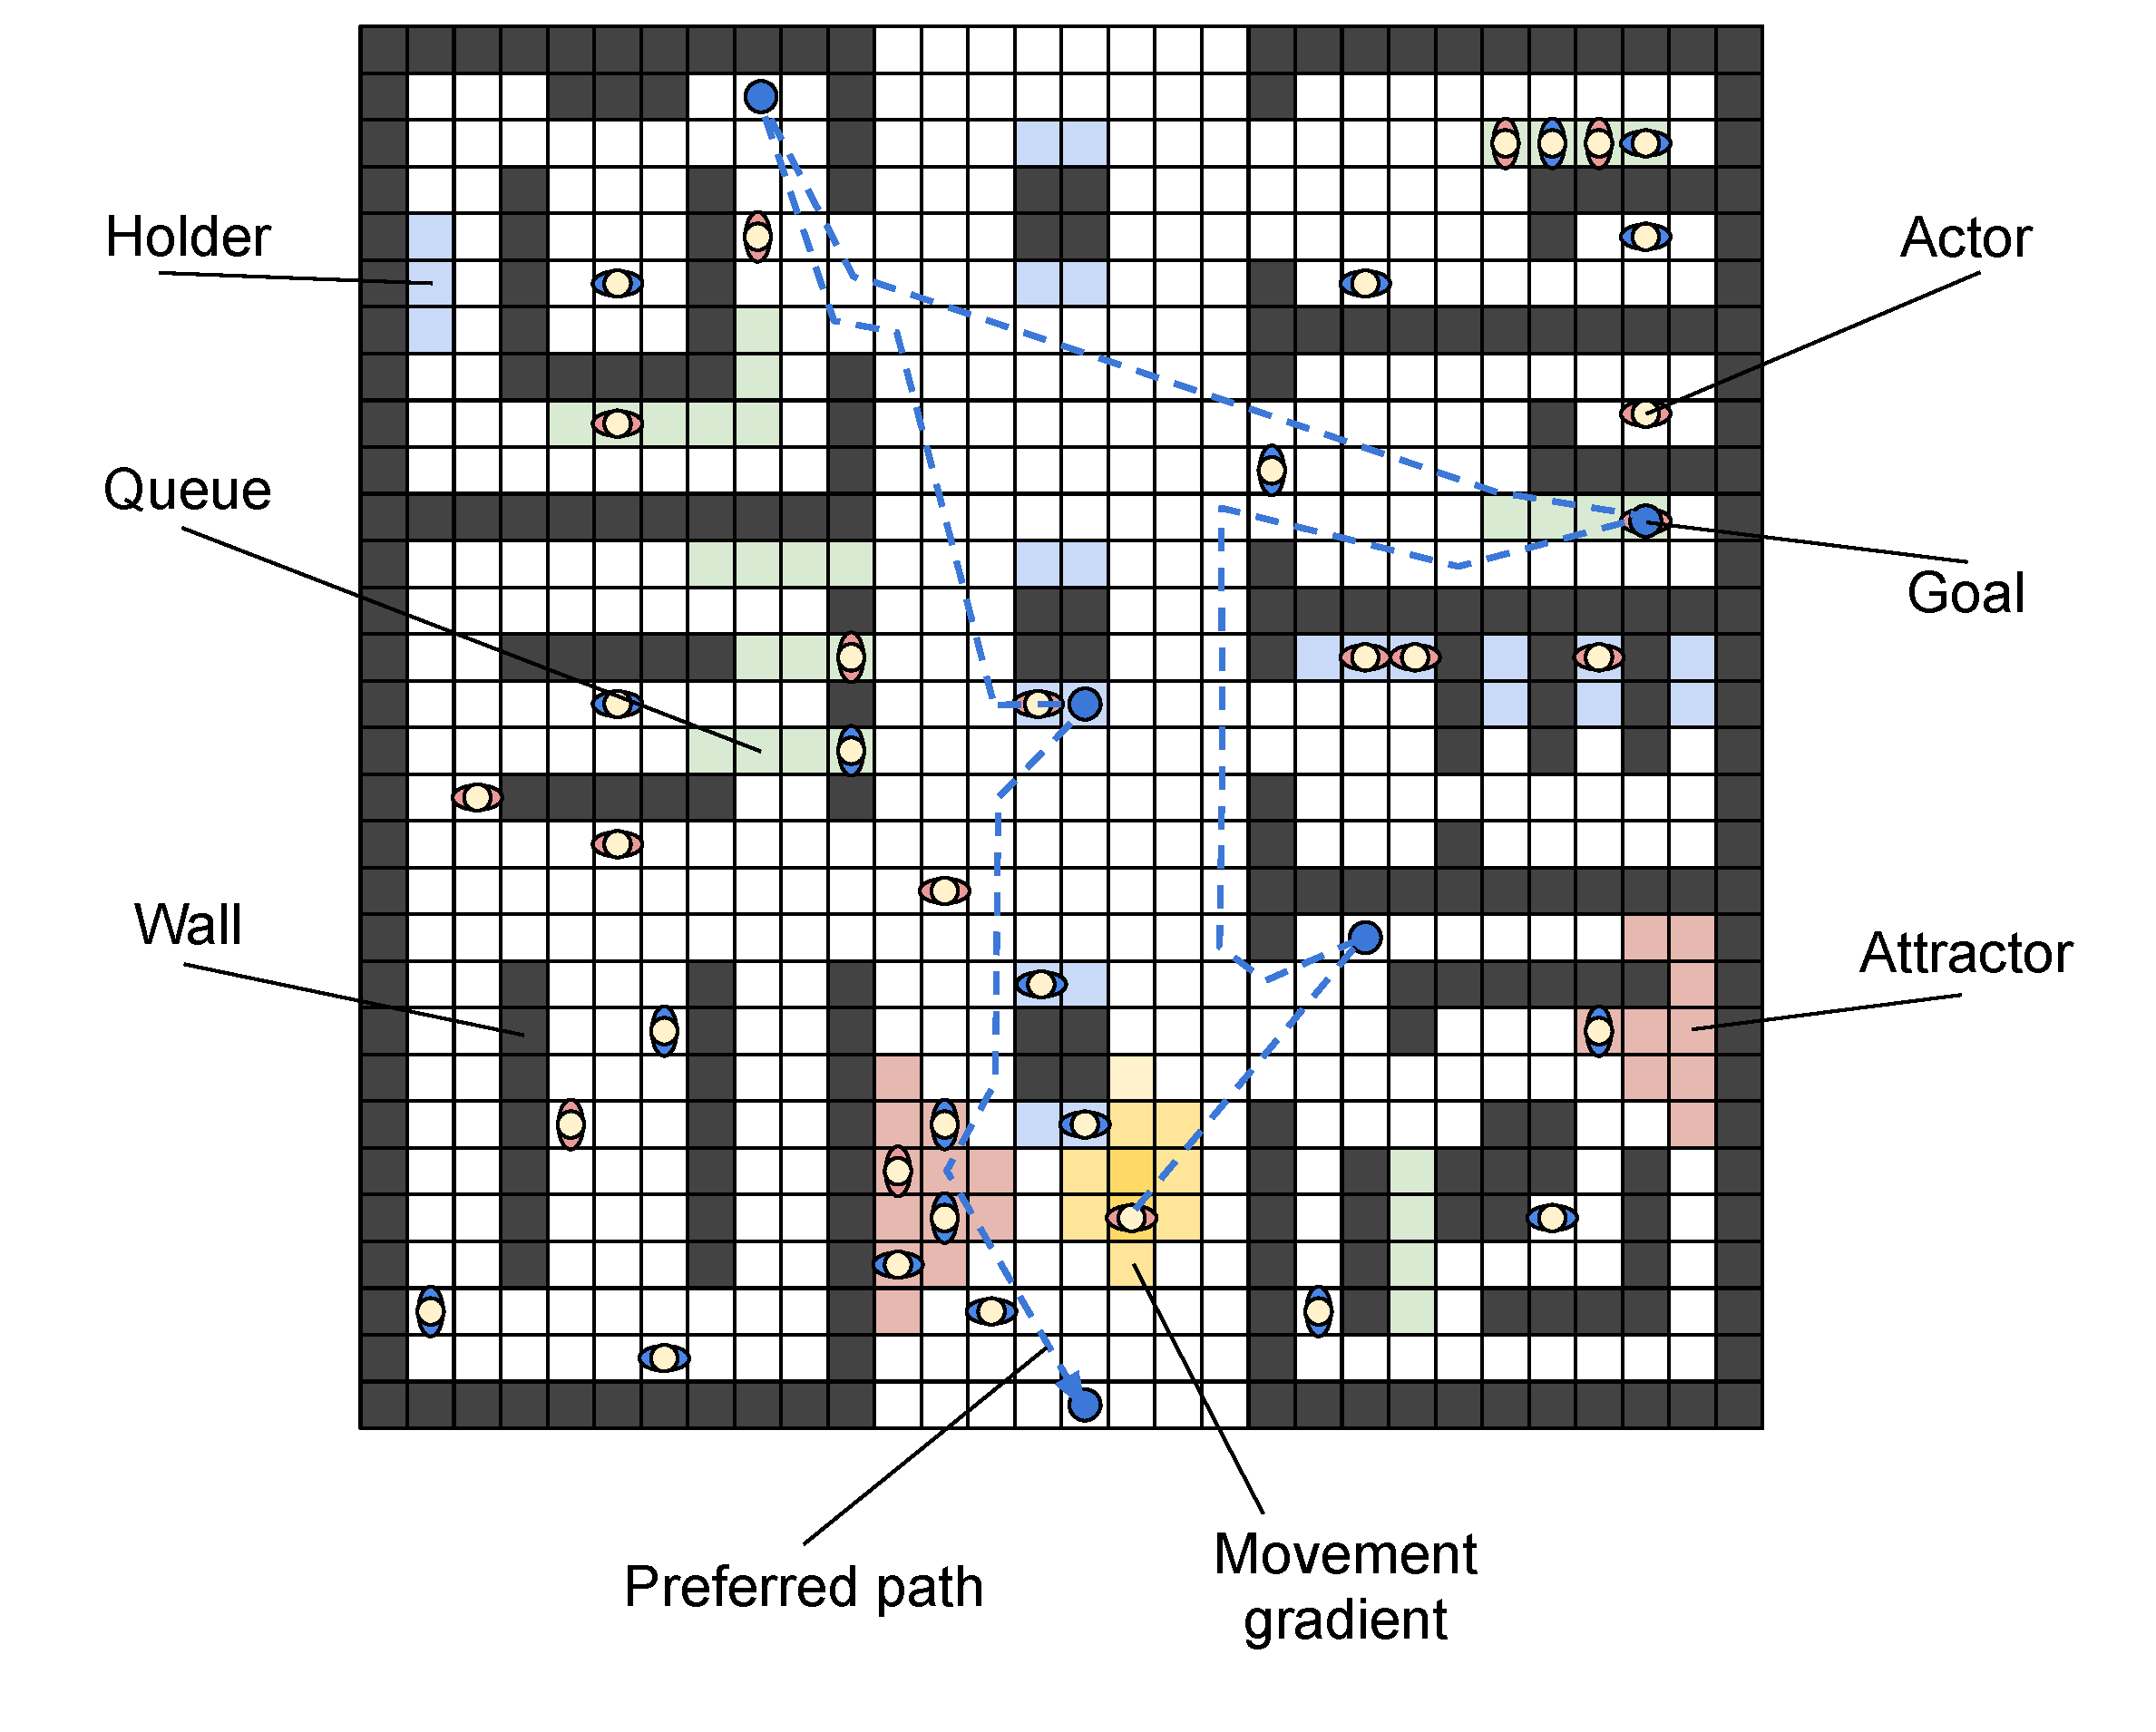
\includegraphics[scale=0.3]{./img/Overview.pdf}
        \caption{Zastosowana dekompozycja problemu.}
        \label{fig:overview}
    \end{figure}

Model centrum handlowego przewiduje istnienie specjalnych stref, wewnątrz których algorytmy odpowiedzialne za poruszanie agentów są modyfikowane lub zastępowane celem modelowania dobrze zdefiniowanych elementarnych zachowań, takich jak \emph{kolejkowanie}, czy \emph{grupowanie się}. W wyniku obserwacji stwierdzono istnienie czterech rodzajów stref specjalnych - strefy przyciągania uwagi (atraktory), kolejki, przejścia i miejsca oczekiwania (opóźniacze).

    \subsection{Atraktory}
    \label{sec:attractors}

Atraktor jest specjalną strefą przyciągającą uwagę agentów poruszających się po centrum handlowym. Atraktor ma za zadanie modelować obecność przedmiotu lub zjawiska, które przykuwa uwagę ludzi na terenie centrum handlowego, a wynikiem jego działania jest spontaniczne powstawanie skupisk ludzi - \emph{grupowanie się}.

    \begin{figure}[H]
        \centering
        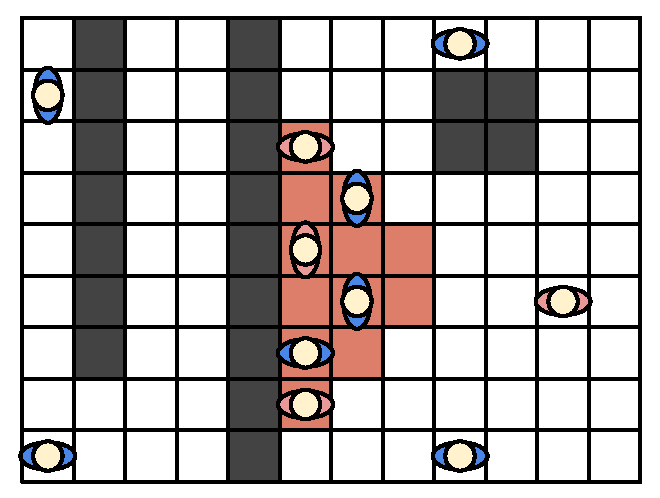
\includegraphics[scale=0.4]{./img/Crowding.pdf}
        \caption{Grupowanie się agentów w obrębie atraktora.}
        \label{fig:crowding}
    \end{figure}

Atraktory różnią się między sobą typami - atraktory różnych typów przyciągają inne rodzaje agentów, co modeluje różnice w preferencjach ludzi przebywających w centrum handlowym.

    \subsection{Kolejki}
    \label{sec:queues}

Drugim istotnym z punktu widzenia modelu centrum handlowego typem strefy specjalnej jest strefa kolejki. Zadaniem kolejki jest modelowanie zjawiska \emph{ścisłego kolejkowania się} ludzi, na przykład przy kasie sklepowej, lub na stopniach eskalatora, co nie wynika z ogólnego modelu ruchu.

    \begin{figure}[H]
        \centering
        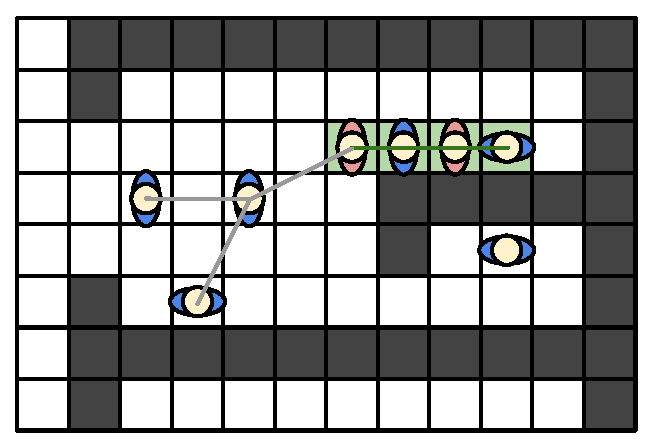
\includegraphics[scale=0.4]{./img/Queueing.pdf}
        \caption{Kolejkowanie się ludzi przy kasie sklepowej z zaznaczoną kolejką ścisłą.}
        \label{fig:queueing}
    \end{figure}

    \subsection{Przejścia/wejścia/wyjścia}
    \label{sec:entrance-exits}

Strefy przejść podobnie jak koleki modyfikują preferencje odległościowe agentów i prowądzą do zmniejszenia odległości między nimi, co nie wynika z ogólnego modelu ruchu. Przejścia, jak sama nazwa wskazuje, modelują wszelkiego rodzaju wejścia, wyjścia i przejścia prowadzące między piętrami centrum handlowego.

    \begin{figure}[H]
        \centering
        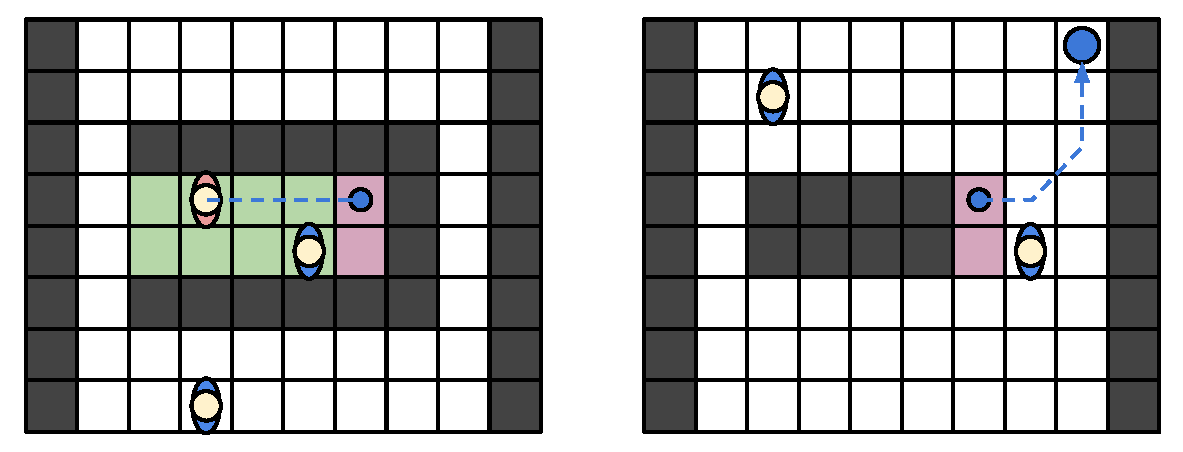
\includegraphics[scale=0.4]{./img/EntranceExits.pdf}
        \caption{Poruszanie się agenta po eskalatorze pomiędzy piętrami centrum handlowego.}
        \label{fig:passing-through}
    \end{figure}

    \subsection{Miejsca oczekiwania (Opóźniacze)}
    \label{sec:holders}

Ostatnim istotnym typem strefy specjalnej jest miejsce oczekiwania, modelujące wszelkiego rodzaju miejsca spędzania czasu w bezruchu.

    \begin{figure}[H]
        \centering
        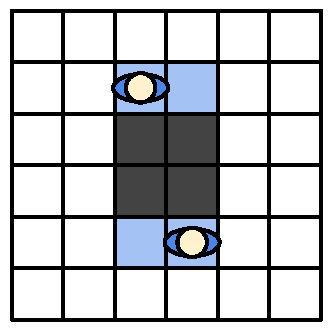
\includegraphics[scale=0.4]{./img/Held.pdf}
        \caption{Agenci oczekujący końca świata.}
        \label{fig:held-down}
    \end{figure}

\newpage
    \section{Model ruchu ludzi}
    \label{sec:move-model}

\noindent
W zastosowanym algorytmie można wyszczególnieć dwie główne, wzajemnie od siebie zależne fazy - fazę \hyperref[sec:tactical]{taktyczną} oraz fazę \hyperref[sec:operational]{operacyjną}, których interakcję przestawiono na poniższym, uproszczonym diagramie.

    \begin{figure}[H]
        \centering
        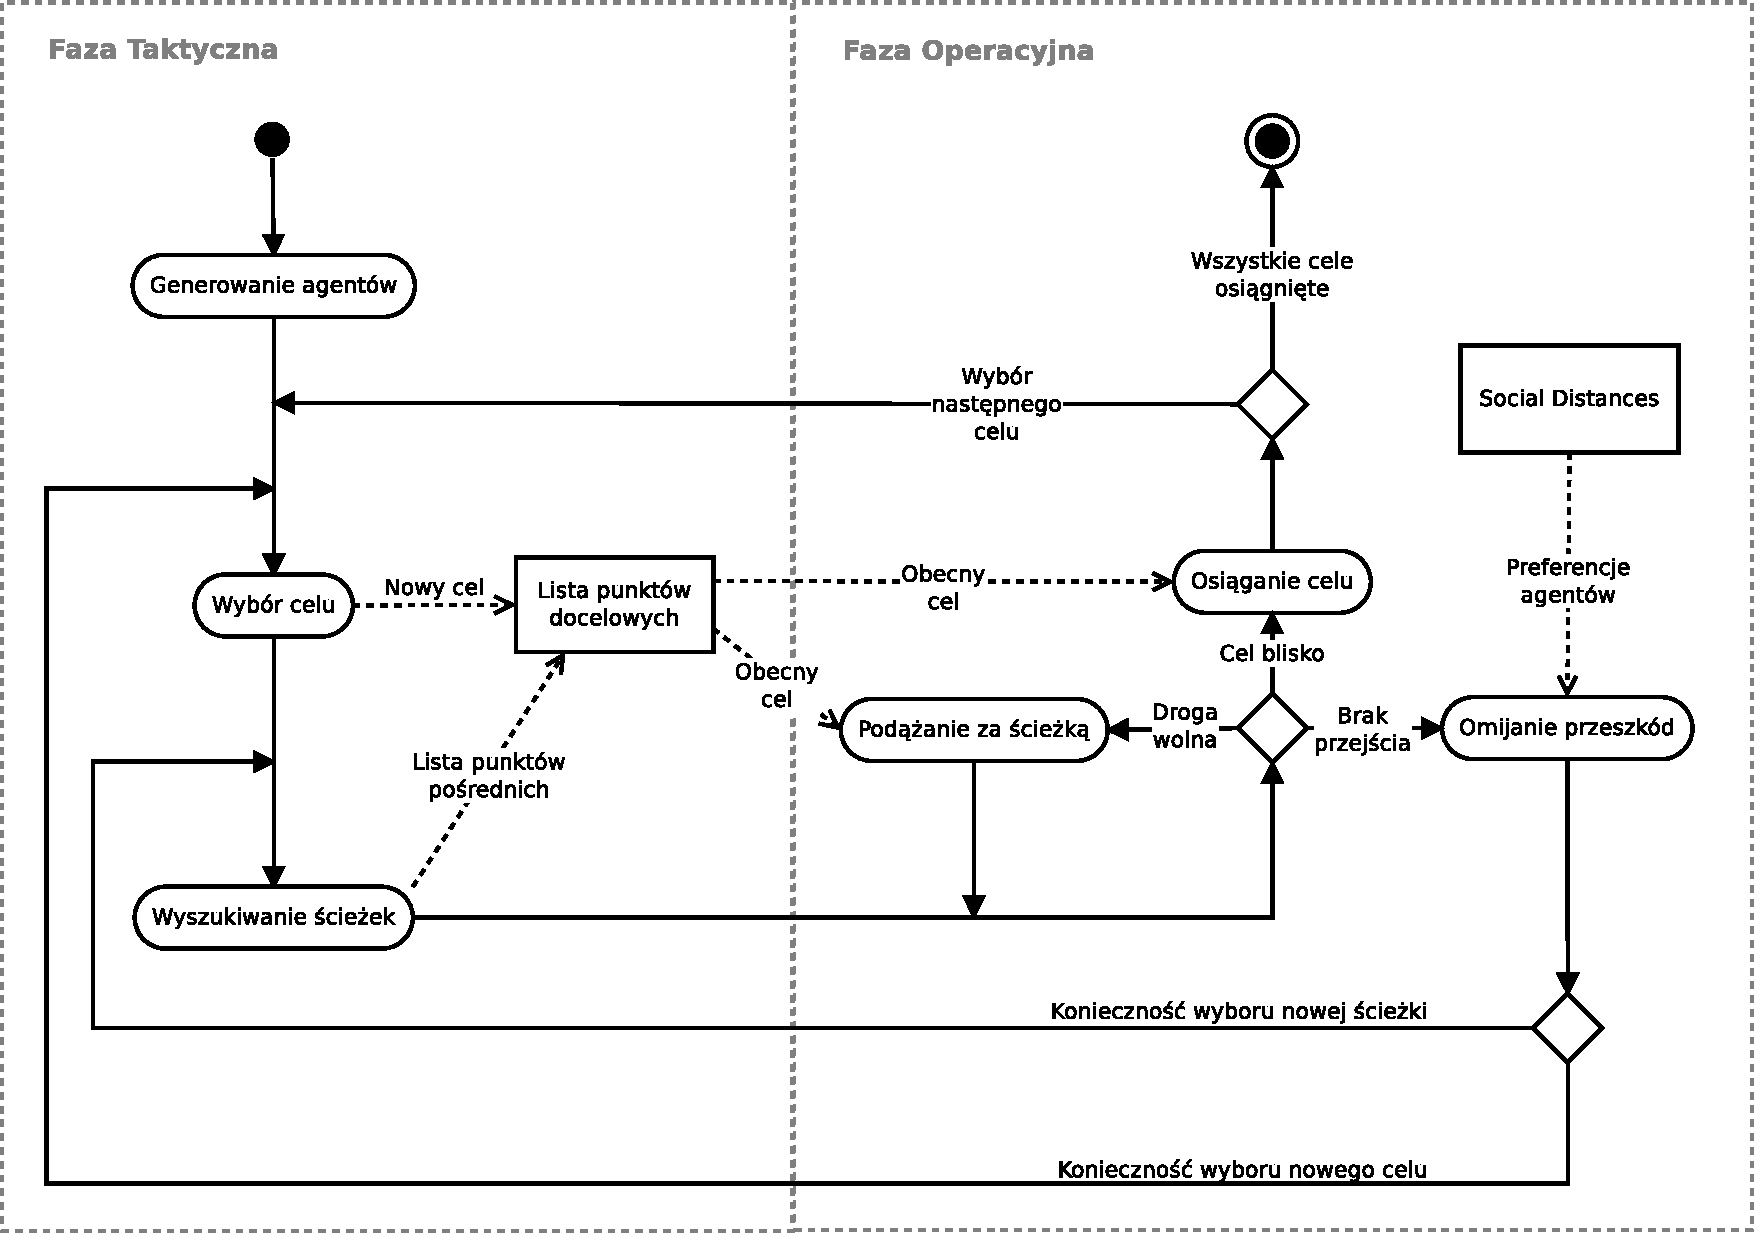
\includegraphics[scale=0.55]{./img/ActorActivity.pdf}
        \caption{Diagram aktywności agentów.}
        \label{fig:actor-activity}
    \end{figure}

Algorytm rozpoczyna działanie od wygenerowania agenta na podstawie wcześniej zdefiniowanych archetypów.
Dla każdego agenta wybierana jest wstępna lista miejsc docelowych, które zostaną przez niego odwiedzone w czasie działania symulacji, oraz obliczana jest optymalna ścieżka łącząca wybrane w poprzednim kroku miejsca docelowe. Algorytm następnie modyfikuje ścieżkę w oparciu o mapę rozkładu stref specjalnych centrum handlowego by lepiej modelować faktyczne zamiary danego agenta. Faza taktyczna kończy się wybraniem niewielkiej ilości punktów pośrednich leżących na wyznaczonej ścieżce.

Po wygenerowaniu niezbędnych danych taktycznych dla każdego agenta algorytm przechodzi do fazy operacyjnej, która odpowiada za właściwe przemieszczanie agentów. Faza ta zachodzi w lokalnym otoczeniu każdego agenta i odpowiada za zachowania takie jak omijanie przeszkód, grupowanie się i podążanie za obraną ścieżką.
Algorytm na podstawie bezpośredniego otoczenia agenta oraz metadanych dotyczących obecnego celu jego podróży podejmuje decyzje o możliwości wykonania ruchu, lub w przypadku skrajnym o modyfikacji wybranej ścieżki prowadzącej do celu, czy nawet zmianie aktualnego celu podróży.
W przypadku osiągnięcia miejsca docelowego algorytm przechodzi do rozpatrywania następnego miejsca docelowego, lub w tryb ``błądzenia'', gdy osiągnięto już wszystkie wyznaczone cele.

\newpage
        \subsection{Faza taktyczna}
        \label{sec:tactical}

        \begin{figure}[H]
            \centering
            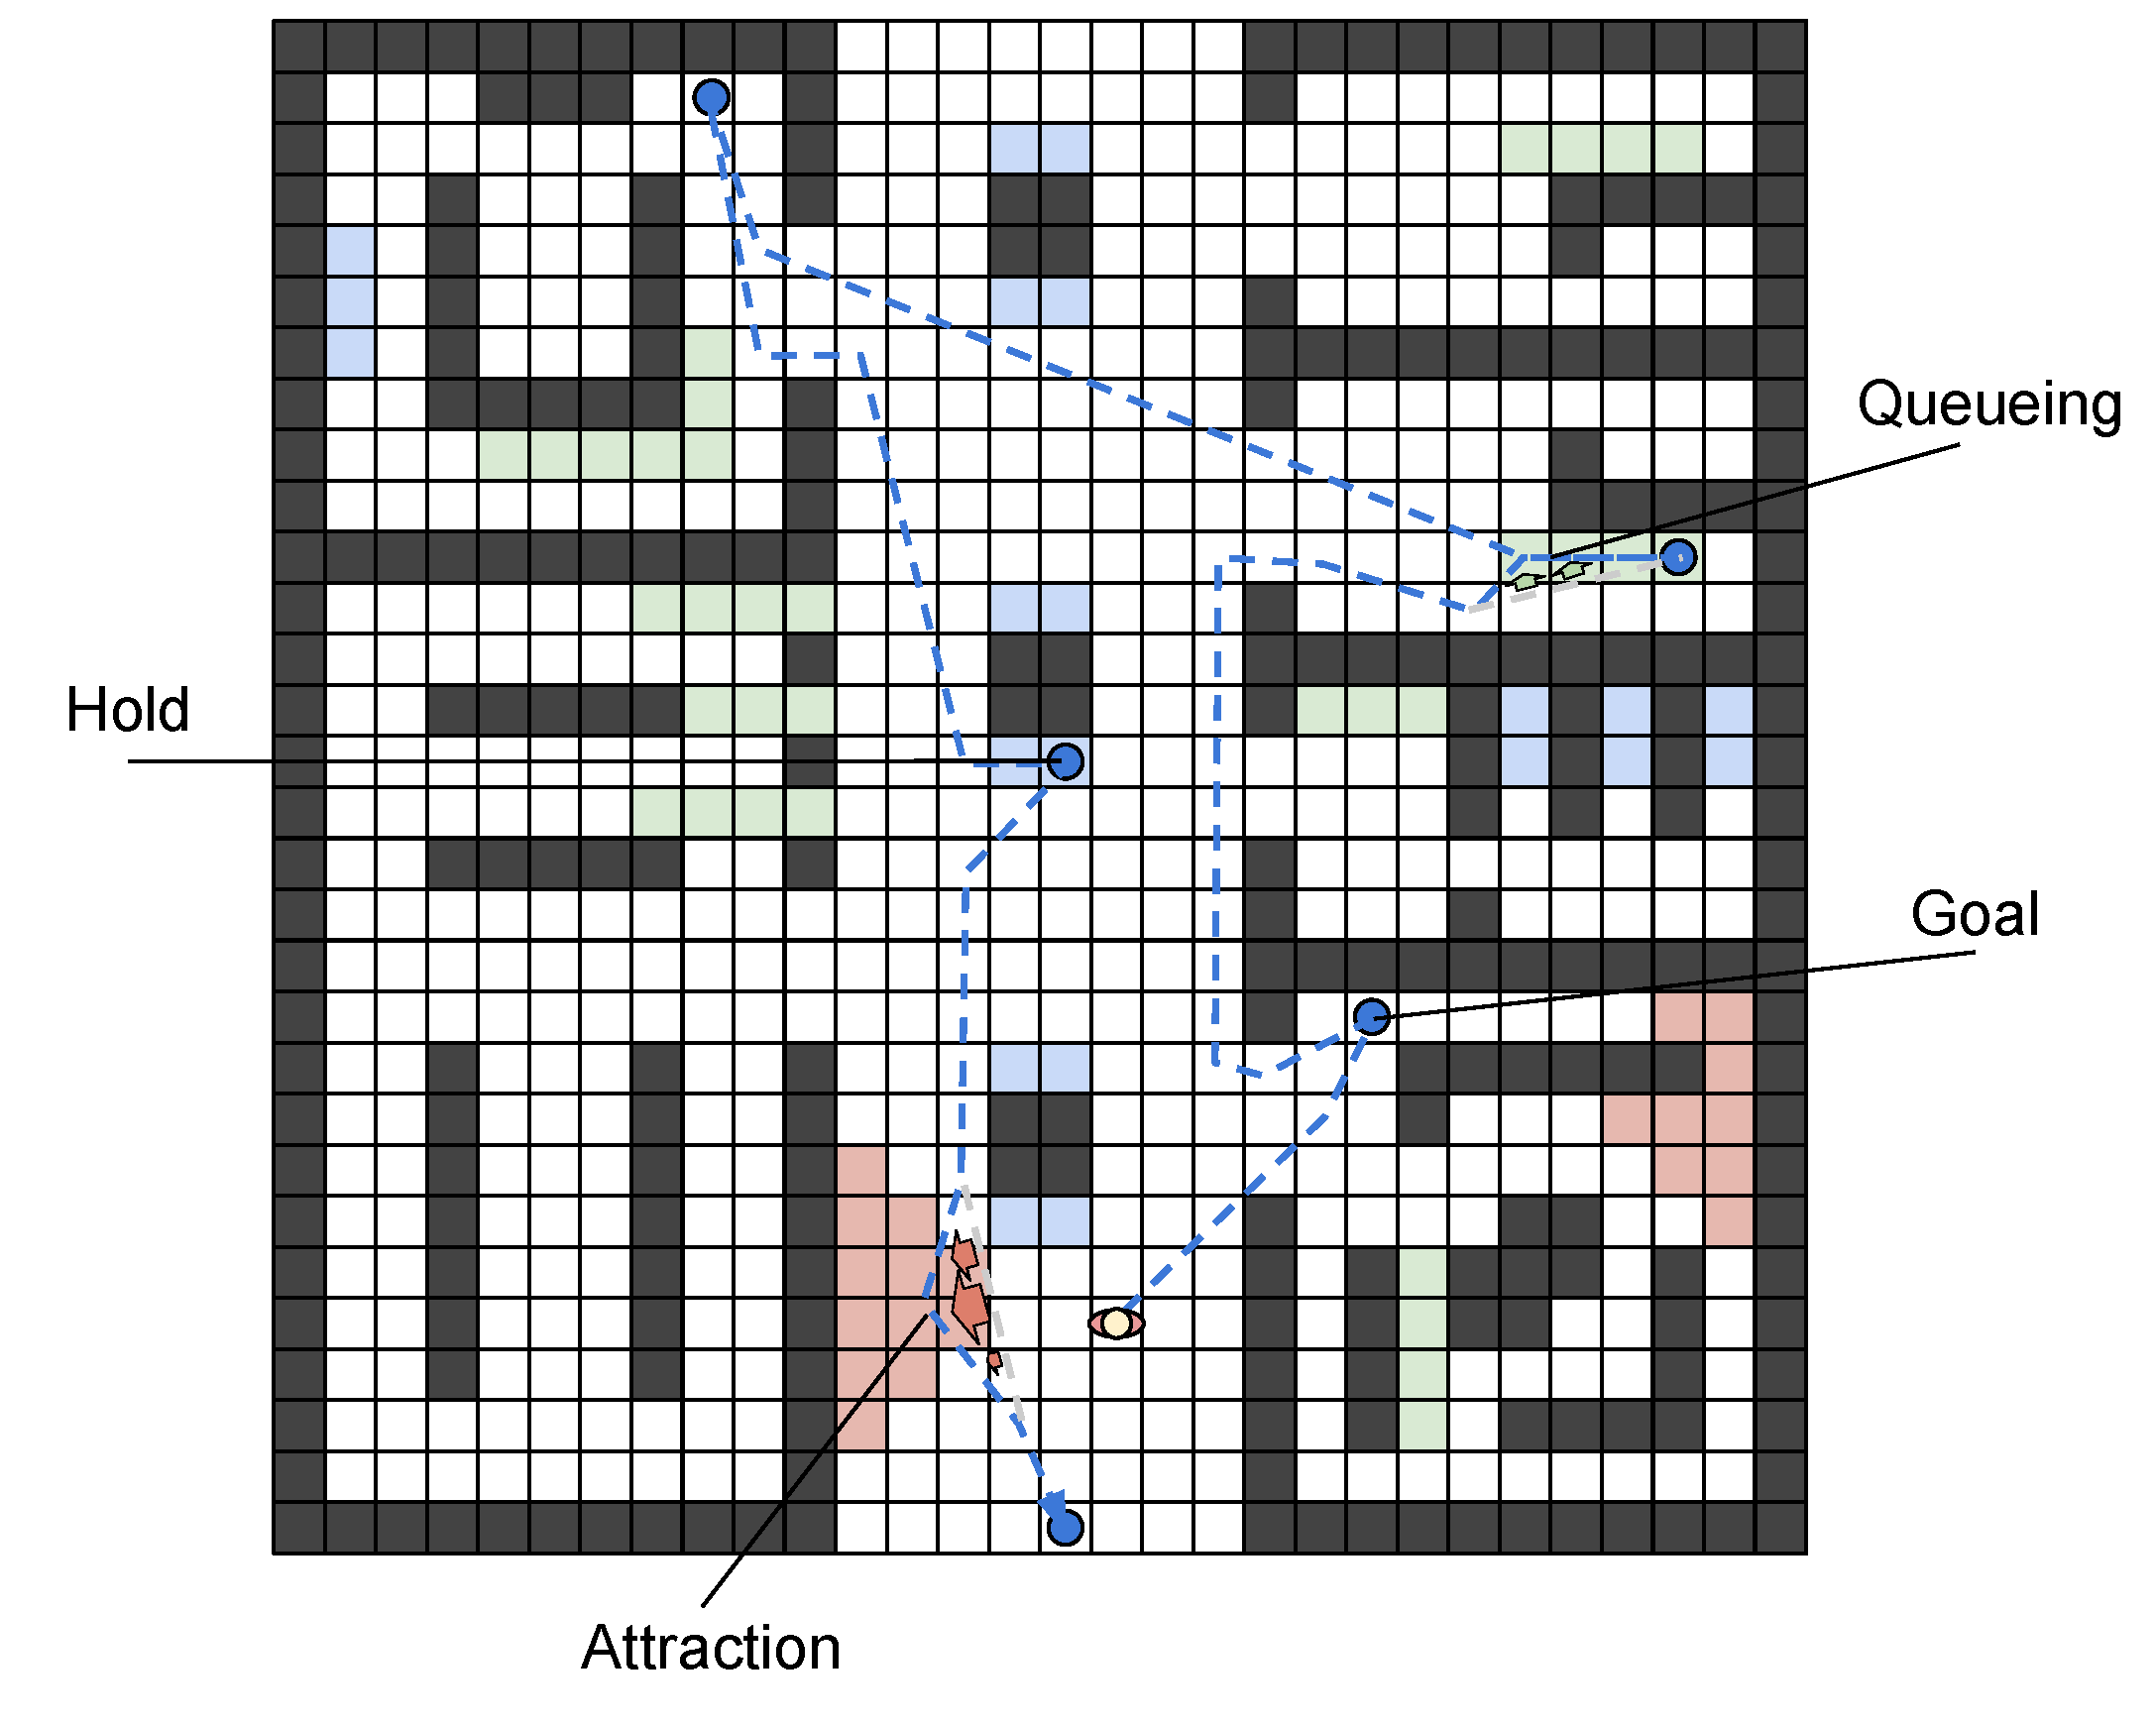
\includegraphics[scale=0.3]{./img/Tactical.pdf}
            \caption{Zakres operacji taktycznej części modelu ruchu.}
            \label{fig:tactical}
        \end{figure}

\noindent
Faza taktyczna zachodzi globalnie dla każdego agenta bez uwzględnienia jego lokalnego otoczenia, innych agentów, czy fizycznych właściwości centrum handlowego - nie jest istotnym, czy dany korytarz został zablokowany przez grupę ludzi i nie umożliwia przejścia. Faza ta modeluje abstrakcyjne zamiary agenta i jej celem jest przede wszystkim wybór listy miejsc docelowych oraz wyznaczenie dróg do nich prowadzących. \\

Osiągnięto to dzięki \hyperref[sec:path-finding]{algorytmowi znajdowania ścieżek A*} oraz \hyperref[sec:mall-impl]{mapie rozkładu stref specjalnych} centrum handlowego, która jest wykorzystywana jako dodatkowa heurystyka A* - specjalne strefy centrum handlowego modyfikują estymowaną ocenę danego punktu wyznaczanej ścieżki nadając jej pożądany kształt i prowadząc ją w odpowiedni sposób do celu podróży. \\

Przy wyznaczaniu ścieżek pod uwagę brane są \hyperref[sec:attractors]{atraktory}, \hyperref[sec:queues]{kolejki} i \hyperref[sec:entrance-exits]{przejścia}, które algorytm stara się uwzględnić za pomocą opisanej heurystyki.

\newpage
        \subsection{Faza operacyjna}
        \label{sec:operational}

        \begin{figure}[H]
            \centering
            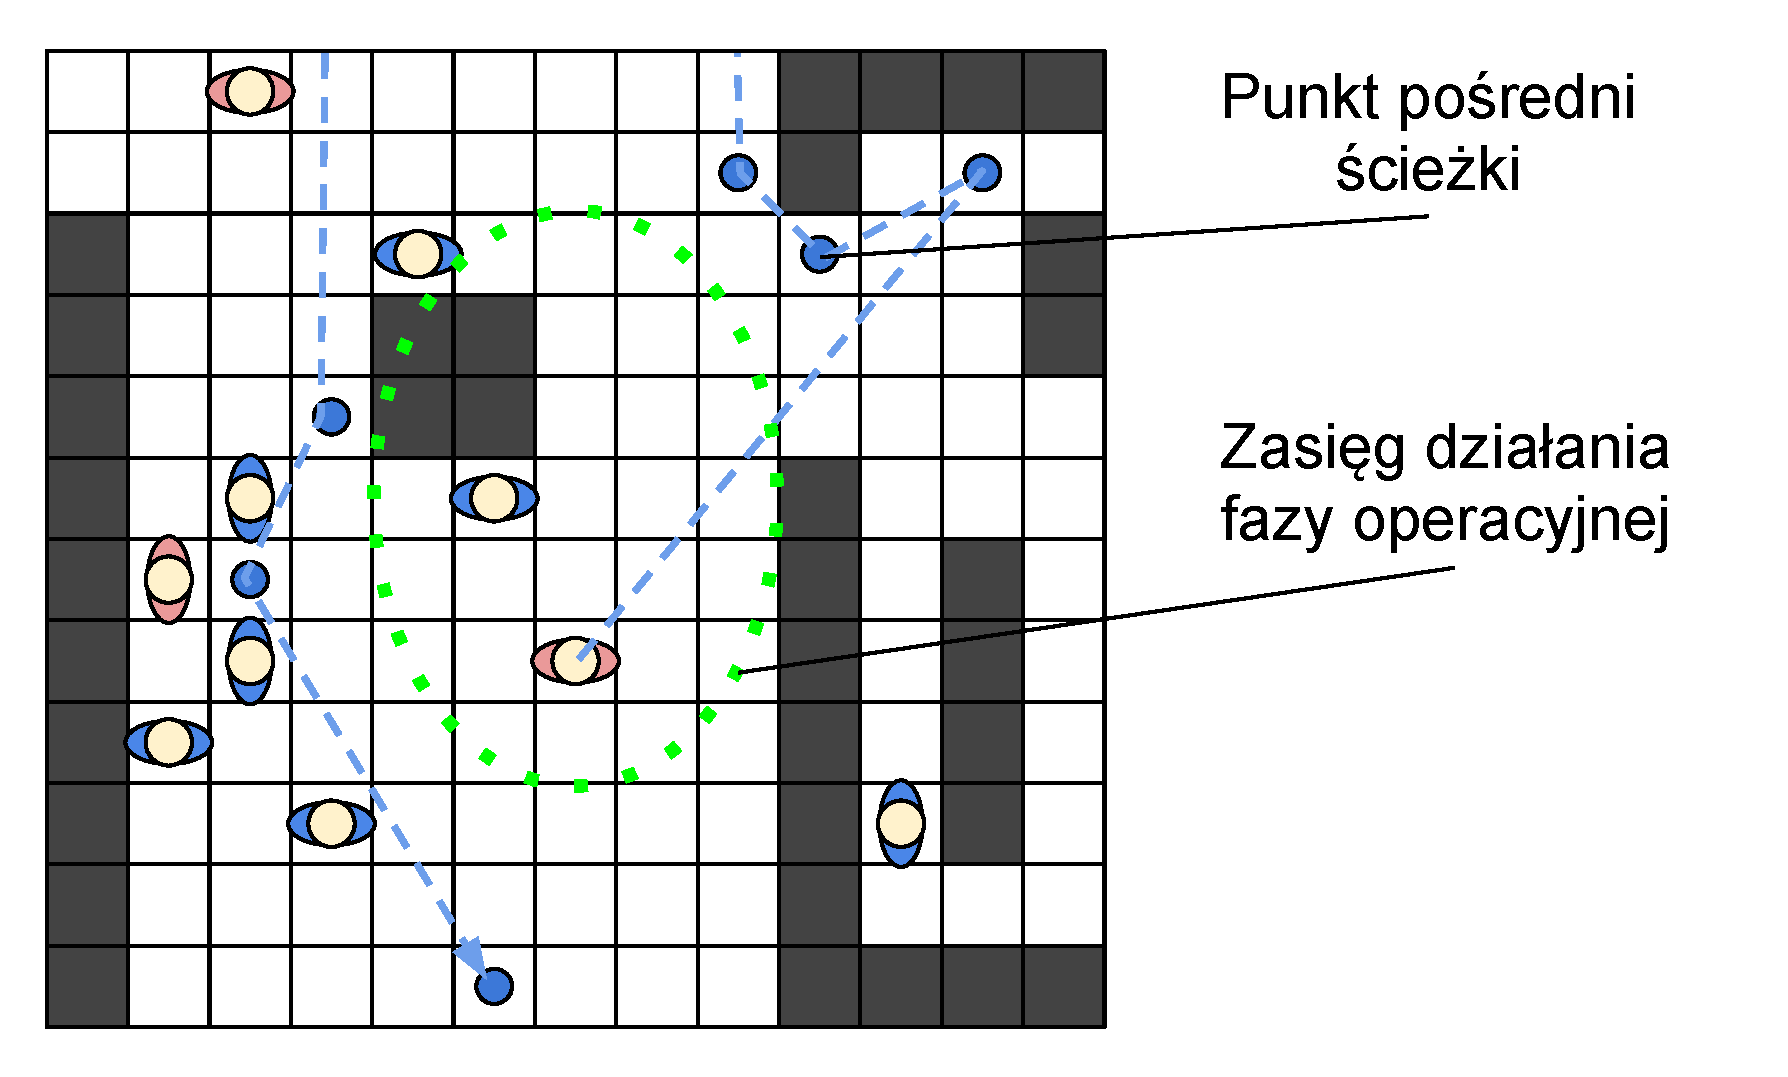
\includegraphics[scale=0.3]{./img/Operative.pdf}
            \caption{Zakres działania operacyjnej części modelu ruchu.}
            \label{fig:operational}
        \end{figure}

        % TODO Potrzeba większego opisu, który bardziej zagłębia się w wybrany algorytm operacyjny.

\noindent
Faza operacyjna zachodzi w lokalnym otoczeniu każdego agenta, a jej celem jest wykonanie właściwego ruchu agenta. Faza ta jest odpowiedzialna za unikanie kolizji i omijanie przeszkód. Pod uwagę brani są inni agenci oraz metadane dotyczące drogi prowadzącej do aktualnego celu podróży wygenerowane w taktyczniej fazie działania algorytmu. W implementacji fazy operacyjnej wykorzystano zmodyfikowane algorytmy \hyperref[sec:movement-impl]{Ped-4} i \hyperref[sec:social-force-impl]{Social-Force}. \\

Oryginalny \textbf{Ped-4} został zaproponowany w pracy \textit{Modeling Four Directional Pedestrian Movements} (\cite{refs:4-way-movement}). Ponieważ prowadzi on do samoorganizowania się pieszych w kolumny, w symulacji galerii używany jest w odniesieniu do przestrzeni, po których ruch odbywa się w sposób uporządkowany (tj. do korytarzy, alejek oraz niewielkich skrzyżowań). \\

\noindent
Algorytm składa się z następujących etapów:
\begin{enumerate}
\item \textbf{Dostosowanie kierunku ruchu} \
    - gdy kąt między kierunkiem ruchu, a kierunkiem do celu przekroczy wartość graniczną, pieszy skręca w stronę celu.
\item \textbf{Zmiana pasa ruchu} \
    - obliczana jest ilość wolnych pól dla obecnie zajmowanego pasa i dla pasów sąsiednich. Pieszy zajmuje ten pas, który na chwilę obecną umożliwia mu przesunięcie się o największą ilość pól do przodu. Przy wyborze preferowany jest dotychczasowy pas. W przypadku, gdy obecnie zajmowany pas nie jest ``czysty'' (tzn. z naprzeciwka idzie inny pieszy), aby uniknać kolizji pieszy stara się ``schować'' za inną osobą idącą w tym samym co on kierunku.
\item \textbf{Krok naprzód} \
    - w przypadku, gdy pole bezpośrednio przed pieszym (zgodnie z kierunkiem ruchu) jest wolne - próba zajęcia go. Jeśli nie jest to możliwe - próba dokonania zamiany miejsca z innym pieszym. Wymiana odzwierciedla sytuację, gdy piesi ``skręcają tułowie'', by ``przecisnąć się'' obok siebie. Etap \textit{krok naprzód} powtarzany jest wielokrotnie, dopóki nie skończą się ``punkty ruchu'' pieszego.
\end{enumerate}

\newpage

\noindent
Poniżej zamieszczono preferowaną kolejność dokonywania zamian:

\begin{enumerate}
\item między pieszymi idącymi w przeciwnych kierunkach na tym samym pasie
\item między pieszymi idącymi w przeciwnych kierunkach na sąsiednich pasach (na polach po przekątnej)
\item między pieszymi idącymi w kierunkach prostopadłych względem siebie (na polach po przekątnej)
\item między pieszymi idącymi w kierunkach prostopadłych względem siebie (jeden ``tarasuje'' drugiemu drogę)
\end{enumerate}

\noindent
Pieszy może wybrać daną możliwość tylko wtedy, gdy jego ``partner'' do zamiany nie wykonał jeszcze swojego ruchu. Jeśli dana wymiana nie dojdzie do skutku, próbowana jest kolejna opcja z listy (znajduje to potwierdzenie w obserwacjach - w sytuacji dużego tłoku ludzie chętniej dokonują takich manewrów). \\

Algorytm \textbf{Social Force} opiera się na obserwacji, że każdy człowiek posiada wokół siebie (głównie przed sobą) tzw. \textit{strefę komfortu}, w której niechętnie widzi osoby postronne. Po zsumowaniu stref komfortu wszystkich agentów otrzymuje się swoisty rozkład potencjału, na podstawie którego wyznaczany jest ich dalszy kierunek ruchu. Zasada, według której odbywa się ruch, jest prosta - dojść do celu po polach o jak najmniejszym potencjale. Jeśli w danym momencie brak jest dostępnych pól, pieszy ``drepcze'' w miejscu w oczekiwaniu na zwolnienie się któregoś z nich. Algorytm \textit{Social Force} służy głównie do modelowania miejsc, w których ludzie ``wałęsają się'', jak place czy wnętrza sklepów.

\newpage
    \section{Implementacja}
    \label{sec:implementation}

    W poniższej sekcji zawarto opis konkretnej implementacji wybranych algorytmów.

        \subsection{Reprezentacja centrum handlowego}
        \label{sec:mall-impl}

        Centra handlowe reprezentowane są za pomocą map bitowych (plików \emph{.bmp}), których piksele kodują odpowiadające im komórki siatki symulacji, co pozwala tworzyć nowe rozkłady pomieszczeń i stref spejcalnych w bardzo prosty i szybki sposób. Implementacja przewiduje istnienie dwóch map dla każdego centrum handlowego - mapę rozkładu pomieszczeń i algorytmów ruchu fazy operacyjnej (rysunek \ref{fig:mall-layout}) oraz mapę rozkładu stref specjalnych centrum handlowego (rysunek \ref{fig:mall-features}).

        \begin{figure}[H]
            \centering
            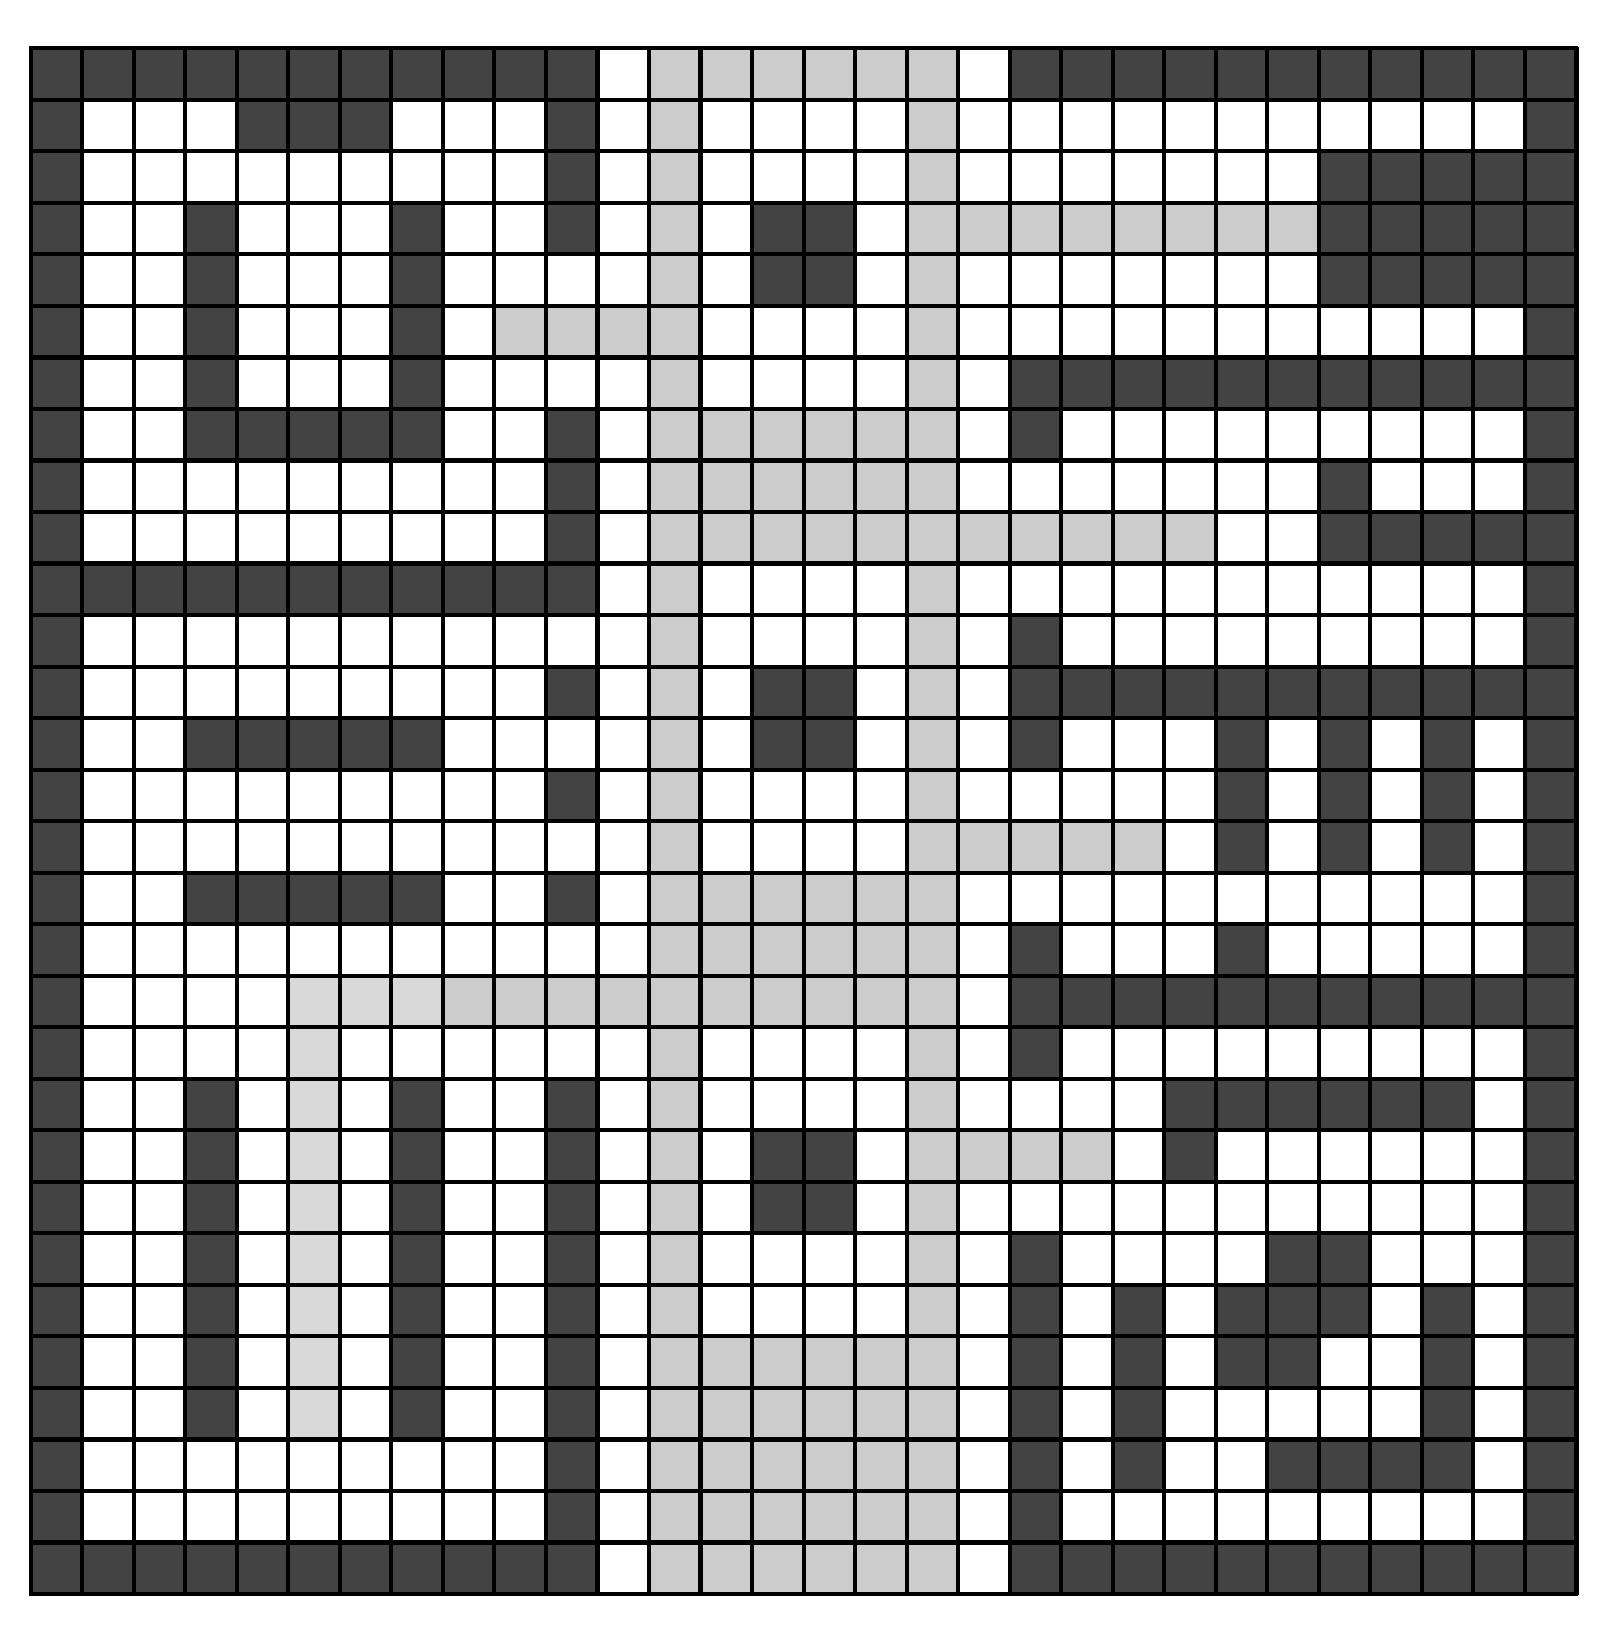
\includegraphics[scale=0.3]{./img/MallLayout.pdf}
            \caption{Przykładowy rozkład pomieszczeń i algorytmów ruchu małego centrum handlowego.}
            \label{fig:mall-layout}
        \end{figure}

        \emph{Mapa rozkładu pomieszczeń} zawiera informacje o fizycznych właściwościach pomieszczeń modelowanego centrum handlowego - usytułówanie ściań i innych obiektów blokujących przejście. Dodatkowo zawarto na niej rozkład algorytmów ruchu wykorzystanych w \hyperref[sec:operational]{fazie operacyjnej}, co pozwala jednoznacznie określić położenie korytarzy, skrzyżowań i innych cech centrum handlowego związanych z ruchem agentów. \\

\noindent
Wartości znaczące poszczególnych pixeli $RGB$ mapy:

        \begin{itemize}
            \item $(0x00, *, *)$ - wartość zarezerwowana dla ścian i innych obiektów blokujących przejście.
            \item $(0x7F, *, *)$ - wartość determinująca wykorzystanie algorytmu \hyperref[sec:movement-impl]{Ped-4}.
            \item $(0xFF, *, *)$ - wartość determinująca wykorzystanie algorytmu \hyperref[sec:social-force-impl]{Social Force}.
        \end{itemize}

        \begin{figure}[H]
            \centering
            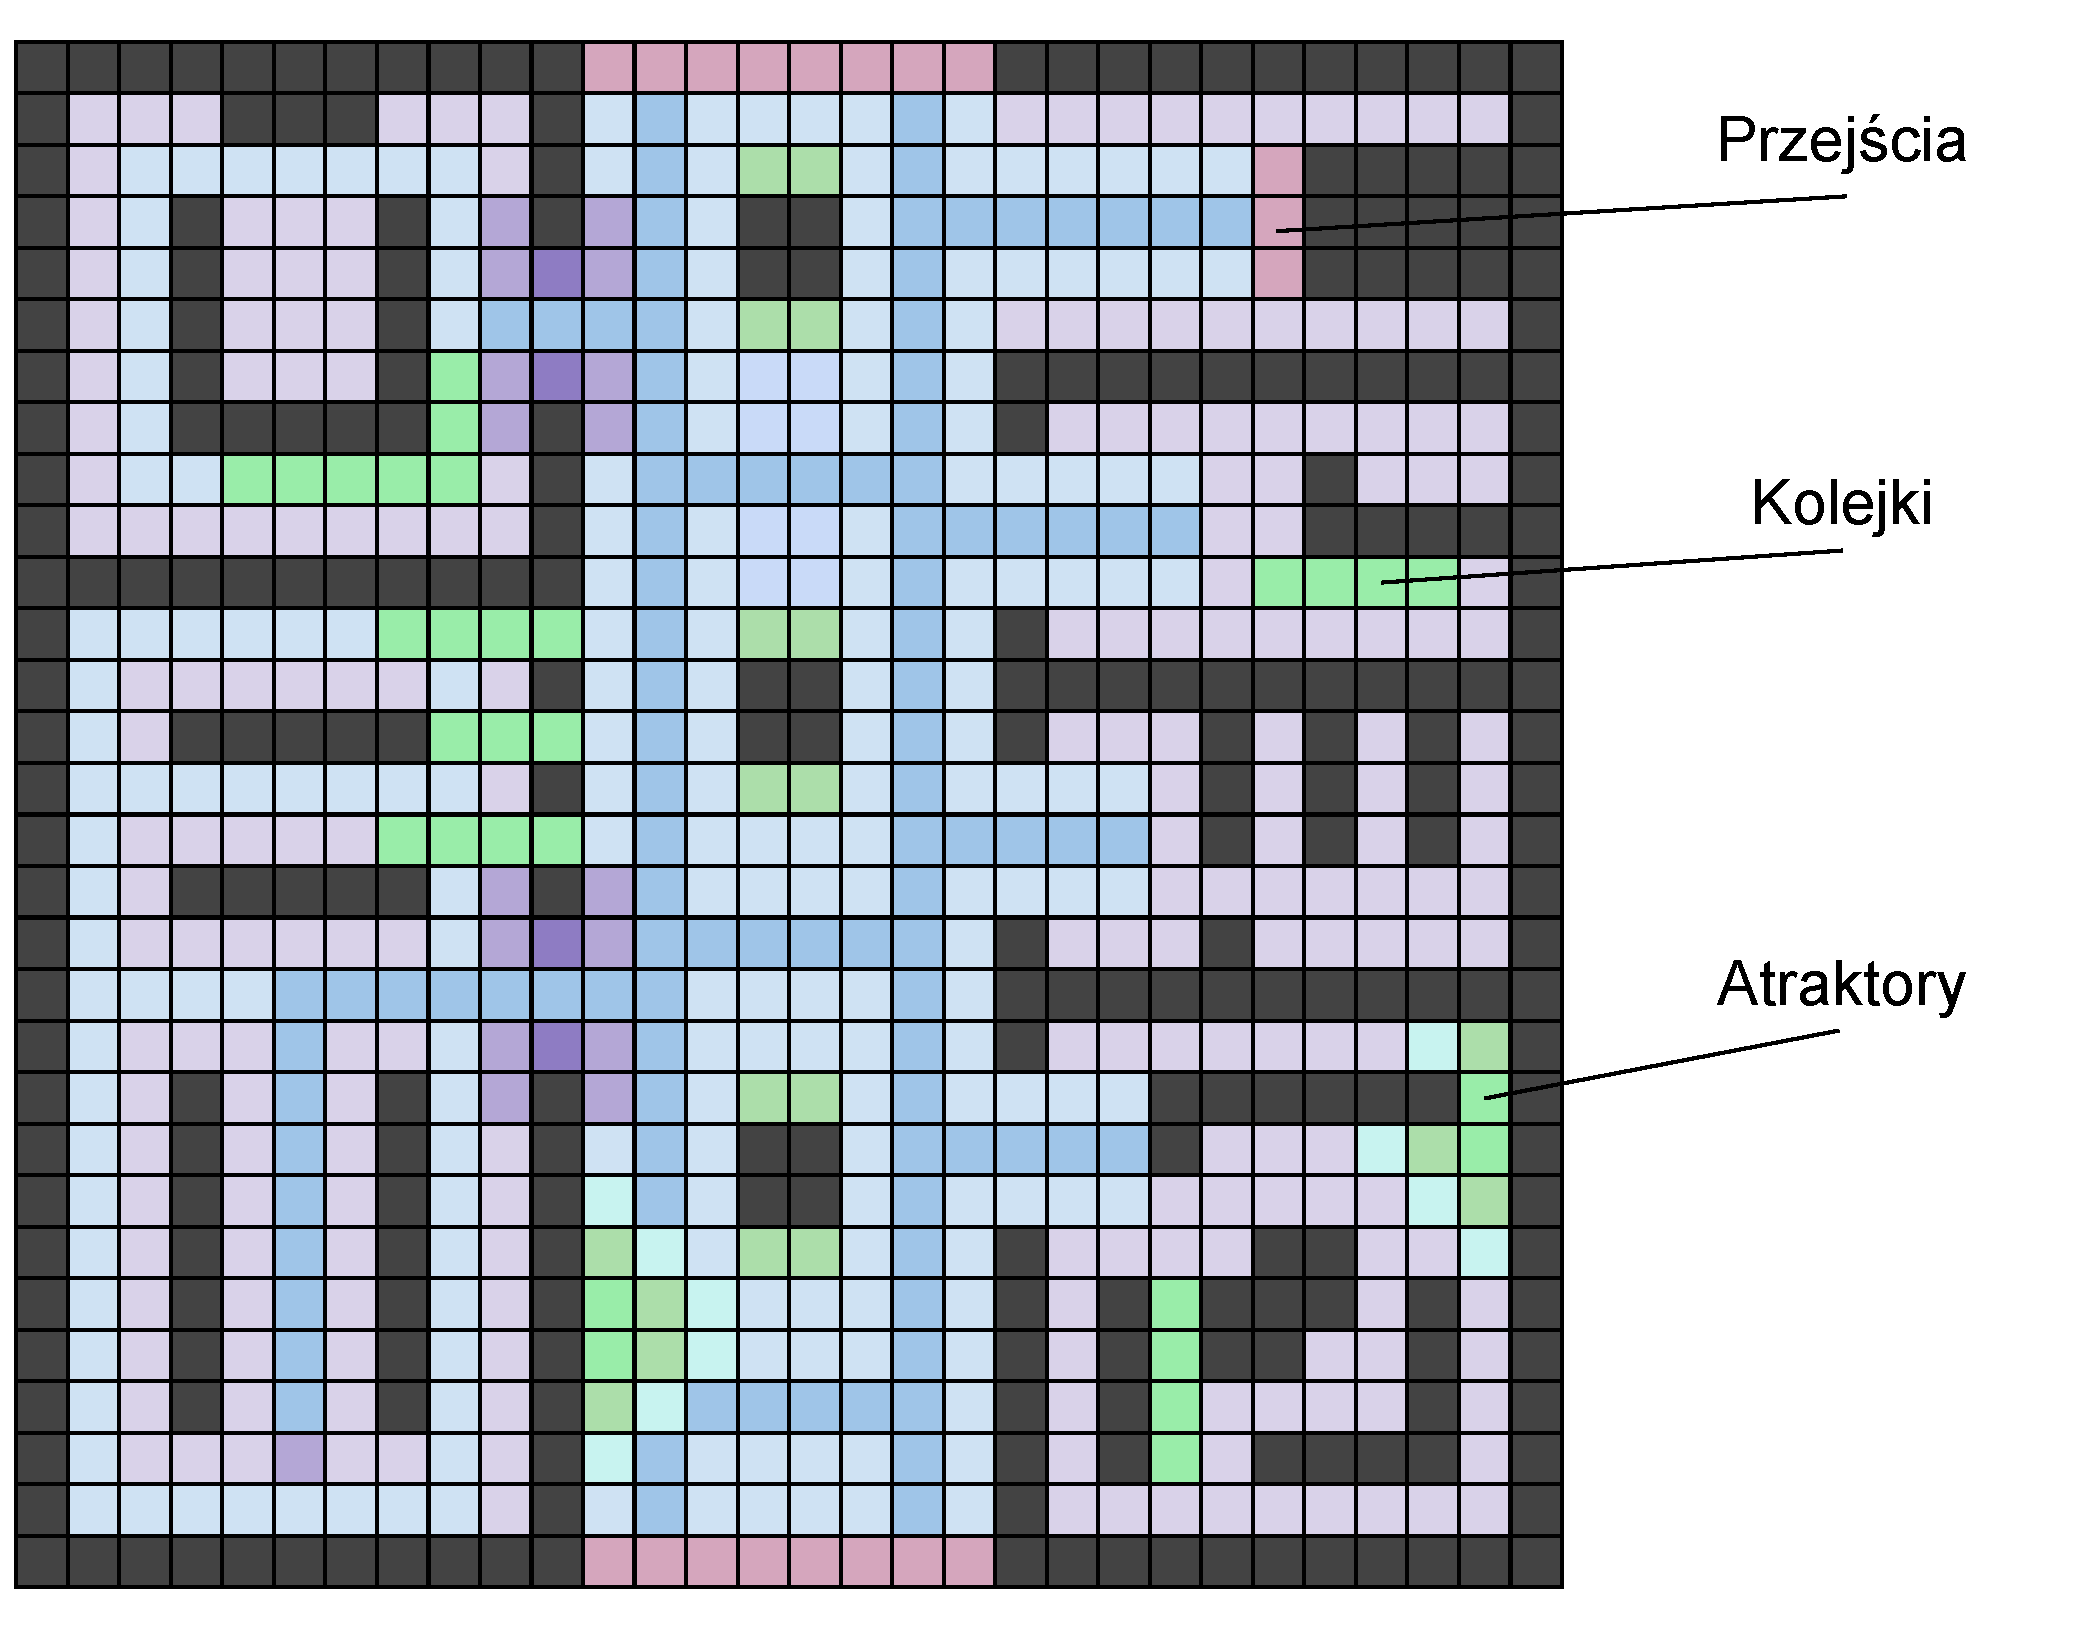
\includegraphics[scale=0.3]{./img/MallFeatures.pdf}
            \caption{Przykładowy rozkład stref specjalnych małego centrum handlowego.}
            \label{fig:mall-features}
        \end{figure}

        \emph{Mapa rozkładu stref specjalnych} centrum handlowego zawiera informacje o funkcjonalnych cechach modelowanego centrum handlowego - rozmieszczenie miejsc przeznaczonych do czekania, kolejek przy kasach sklepowych, okien wystawowych i sieci routingu ułatwiającej przemieszczanie się w centrum handlowym. Informacje te wykorzystywane są przede wszystkim przez \hyperref[sec:tactical]{fazę taktyczną} wykorzystanego algorytmu, gdzie są służą jako \hyperref[sec:path-deviation]{dodatkowa heurystyka} \hyperref[sec:path-finding]{algorytmu wyszukiwania ścieżek A*}. \\

\noindent
Wartości znaczące poszczególnych pixeli $RGB$ mapy:

        \begin{itemize}
            \item $(0x7F, A, H)$ - wartość oznaczająca \hyperref[sec:path-deviation]{uogólniony atraktor} o \emph{atrakcyjności} $A$ i \emph{czasie wstrzymania} $H$.
            \item $(0xFF, *, *)$ - wartość oznaczająca \hyperref[sec:entrance-exits]{przejścia/wejścia}, które odpowiednio tworzą lub usuwają agentów z symulacji.
        \end{itemize}

\noindent
Z racji ograniczonego czasu i niższego priorytetu implementacja nie uwzględnia istnienia wielu pięter w centrum handlowym - symulacja ruchu ludzi wewnątrz wielopiętrowego centrum handlowego może być traktowana jako wiele symulacji ruchu ludzi wewnątrz jednopiętrowego centrum handlowego.

        \subsection{Wybór puntków docelowych}
        \label{sec:destination-choice}

        \emph{Punkty docelowe} reprezentują cele podróży agentów. Z racji mniejszego priorytetu i braku czasu algorytm wybiera zadaną ilość losowych miejsc znajdujących się we wnętrzu centrum handlowego, które następnie sortuje celem minimalizacji sumarycznej długości drogi je łączącej. Opisany sposób wyboru miejsc docelowych pozwala symulować wszystkie zachowania poruszających się ludzi na poziomie lokalnym (na przykład kolejkowanie się) i większość schematów zachowań tłumu na poziomie globalnym (z wyłączeniem bardziej abstrakcyjnych zachowań uwarunkowanych socjologicznie i kulturowo, takich jak różne stosunki ilościowe agentów danego typu w różnych częściach centrum handlowego).

\newpage
        \subsection{Znajdowanie ścieżek}
        \label{sec:path-finding}

W celu wyznaczania ścieżek prowadzących do punktów docelowych wykorzystano algorytm \textbf{A*}. A* jest algorytmem kompletnym, służącym do wyznaczania najkrótszej drogi łączącej dwa wierzchołki grafu, który w każdym przypadku jest w stanie znaleźć drogę, jeśli takowa istnieje. A* wykorzystuje \hyperref[sec:path-deviation]{heurystykę}, która estymuje koszt ścieżki prowadzącej z danego wierzchołka do celu, starając się rozpatrywać tylko najbardziej obiecujące wierzchołki. \\

\noindent
Algorytm przochowuje zbiory wierzchołków ``otwartych'' i ``zamkniętych'', czyli odpowiednio, wierzchołków, które są rozpatrywane i tych, które już zostały sprawdzone. Działanie algorytmu rozpoczyna się od dodania aktualnej pozycji agenta do zbioru wierzchołków otwartych. W każdym następnym kroku algorytm wykonuje iteracyjnie następujące operacje:

        \begin{itemize}
            \item Ze zbioru wierzchołków otwartych wybierany jest najbardziej obiecujący wierzchołek $x$, minimalizujący funkcję $f(x)$:
              \[ f(x) = g(x) + h(x) \]
              gdzie $g(x)$ określa długość drogi prowadzącej z wierzchołka początkowego do wierzchołka $x$, a $h(x)$ określa przewidywaną przez heurystykę długość drogi łączącej wierzchołek $x$ i cel podróży.
            \item W przypadku osiągnięcia punktu docelowego algorytm kończy się sukcesem.
            \item W przeciwnym przypadku wierzchołek $x$ dodawany jest do zbioru wierzchołków zamikniętych, a sąsiadujące z nim wierzchołki (wierzchołki osiągalne w jednym kroku zaczynając w $x$), które nie należą do zbioru wierzchołków zamkniętych, dodawane są do zbioru wierzchołków otwartych.
        \end{itemize}

\noindent
Zależnie od zastosowanej heurystyki algorytm A* jest w stanie dostarczać optymalne ścieżki łączące dwa punkty lub suboptymalne ścieżki, które są obliczane szybciej. Ze względu na rozwiązywany problem i brak wymogu dostarczania optymalnych ścieżek w implementacji zastosowano złożoną, dopuszczalną (\emph{ang. admissible}) heurystykę opisaną w następnej sekcji, którą dodatkowo obarczono wagą $\epsilon = 5$, co pozwala szybko generować ścieżki o pożądanym i koszcie nie przekraczającym $\epsilon$ razy kosztu ścieżki optymalnej.

        \subsection{Dewiacja ścieżek}
        \label{sec:path-deviation}

        Dewiacja ścieżek zachodzi podczas działania algorytmu wyszukiwania ścieżek opisanego w poprzedniej sekcji celem ułatwienia zachodzenia pewnych zachowań, takich jak poruszanie się w odpowiedni sposób po korytarzach centrum handlowego. Odpowiednia dewiacja ścieżek została osiągnięta przez modyfikację heurystyki zastosowanego algorytmu A* - każdy fragment \hyperref[fig:mall-features]{mapy rozkładu stref specjalnych} centrum handlowego posiada przypisaną mu wartość determinującą parametry \textbf{uogólnionego atraktora} - \emph{atrakcję A} oraz \emph{czas wstrzymania H}. \\

        \emph{Atrakcja} odpowiada za przyciąganie agentów do pewnych stref centrum handlowego i ma za zadanie przede wszystkim umożliwić realizację zdefiniowanych przy analizie problemu \hyperref[sec:attractors]{atraktorów}. Jej wartość kodowana jest przez komponent $G$ pixeli $RGB$ mapy rozkładu stref specjalnych centrum handlowego, kodujących atraktory (komponent $R$ równy $0x7F$). Wartość komponentu $G$ należy podzielić przez $0x7F$ celem przeskalowania do przedziału $[0, 2)$. Heurystyka algorytmu A* wykorzystuje tę wartość, jako dodatkowy mnożnik estymowanego kosztu ścieżki, toteż wartość 0 oznacza najsilniejszą atrakcję, wartość 1 brak atrakcji natomiast wartość 2 oznacza odpychanie - algorytm wyszukiwania ścieżek będzie preferował inne drogi.

        \emph{Czas wstrzymania} odpowiada za opóźnianie agentów podczas wykonywania ruchu - agent osiągający komórkę siatki symulacji obarczoną czasem oczekiwania zostaje opóźniony na zadaną ilość czasu. Wartość czasu wstrzymania kodowana jest przez komponent $B$ pixeli $RGB$ mapy rozkładu stref specjalnych centrum handlowego, kodujących atraktory. Wartość tego komponentu traktowana jest jako ilość kroków symulacji, na które opóźniany agent zostanie wstrzymany. \\

Implementacja \emph{uogólnionego atraktora} okazała się na tyle elastyczna, że wyeliminowała konieczność osobnej implementacji \hyperref[sec:queues]{kolejek} i \hyperref[sec:holders]{opóźniaczy} - kolejki realizowane są jako linie znacząco zwiększonej atrakcji o krótkim czasie wstrzymania, natomiast opóźniacze są punktami o znacząco zwiększonym czasie wstrzymania. \hyperref[sec:attractors]{Atraktory} zostały zrealizowane jako gradienty zwiększającej się atrakcji i czasu wstrzymania - agenci odwiedzajacy atraktor spędzają w nim tym więcej czasu, im bliżej jego centrum się znajdują. Dodatkowym atutem zastosowanej implementacji jest możliwość routingu agentów w centrum handlowym. Wszystkie formy stref specjalnych wyrażonych przez modyfikację heurystyki algorytmu A* zostały zawarte na poglądowym rysunku \ref{fig:mall-features}.

        \subsection{Reprezentacja agentów}
        \label{sec:actor-impl}

        Na chwilę obecną agenci opisywani są przez parametry wpływające tylko i wyłącznie na ich ruch w fazie operacyjnej. Docelowo planowane jest rozszerzenie ich zachowania o preferencje dotyczące odwiedzanych miejsc, czasu spędzanego w galerii itp.

    \begin{figure}[H]
        \centering
        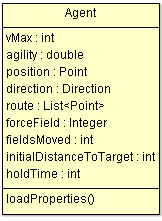
\includegraphics[scale=0.75]{./img/agent.png}
        \caption{Klasa agenta}
        \label{fig:agent}
    \end{figure}

\noindent
Znaczenie poszczególnych parametrów:
\begin{itemize}
\item \textbf{vMax} – maksymalna ilość punktów ruchu do wykorzystania w danej iteracji fazy operacyjnej
\item \textbf{agility} – skłonność do dokonywania zamian z innymi podczas etapu poruszania agentów
\item \textbf{position} – położenie agenta na planszy galerii
\item \textbf{direction} – aktualny kierunek ruchu (dostępne kierunki są zgodne ze stronami świata)
\item \textbf{route} – lista współrzędnych płytek-celów do odwiedzenia
\item \textbf{forceField} – opis wartości potencjału pól wokół agenta (przy założeniu, że agent zwrócony jest w kierunku północnym)
\item \textbf{fieldsMoved} – odległość (mierzona w płytkach) przebyta od ostatniego celu do danej chwili
\item \textbf{initialDistanceToTarget} – teoretyczna minimalna odległość od poprzedniego do obecnego celu
\item \textbf{holdTime} – pozostały czas oczekiwania (np. w kolejce)
\end{itemize}

Część spośród powyższych parametrów agenta inicjalizowana jest na podstawie plików zawierających opisy pewnych ogólnych charakterystyk ludzi, np. "typ dynamiczny" oznacza człowieka poruszającego się szybko i skłonnego do dokonywania zamian, "typ emeryta" oznacza stateczny krok i niechęć do zamian.

        \subsection{Ruch agentów i Ped-4}
        \label{sec:movement-impl}

\noindent
Faza operacyjna składa się z czterech wykonywanych w pętli etapów, co zilustrowano na poniższym schemacie:

    \begin{figure}[H]
        \centering
        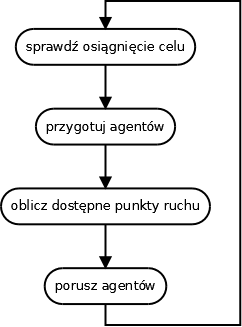
\includegraphics[scale=0.5]{./img/mainloop.png}
        \caption{Pętla fazy operacyjnej}
        \label{fig:operloop}
    \end{figure}

\indent Sprawdzanie osiągnięcia celu służy wyznaczeniu kolejnego celu, o ile poprzedni został osiągnięty. Cel można osiągnąć na dwa sposoby: wchodząc bezpośrednio na płytkę o zadanych współrzędnych bądź wchodząc na płytkę w sąsiedztwie celu (w tym przypadku prawdopodobieństwo uznania celu za osiągnięty zależy od odległości płytki od niego). Po wyznaczeniu nowego celu aktualizowane są parametry wykorzystywane przez algorytmy ruchu, jak początkowa (teoretyczna) minimalna odległość od celu. \newline
\indent Przygotowanie agentów polega na wywołaniu dla każdego z nich metody \emph{prepare()} algorytmu przypisanego do płytki, na której agent aktualnie się znajduje. \newline
\indent Obliczanie dostępnych w danym obiegu fazy iteracyjnej punktów ruchu to przepisanie aktualnej prędkości maksymalnej każdego z agentów. \newline
\indent W etapie poruszania agentów agenci rozpatrywani są cyklicznie. W jednej iteracji (``kroku'') każdy z agentów może wykonać tylko jedną akcję,  np. czkać bądź przemieścić się o jedno (!) pole. Dzięki takiemu rozwiązaniu żaden z agentów nie jest faworyzowany przy dostępie do pól.

\begin{algorithm}
\caption{Faza operacyjna}
\label{alg2}
\begin{algorithmic}
\Procedure{operation\_phase}{}
    \ForAll{agent w galerii}
    \Comment{sprawdź osiągnięcie celu}
        \If{agent osiągnął cel OR agent uznał, że osiągnął cel}
            \State pobierz kolejny cel z listy
            \State zapisz statystyki dotyczące dalszej drogi
        \EndIf
    \EndFor
    \newline
    \ForAll{agent w galerii}
    \Comment{przygotuj agentów}
        \State \textbf{call} Algorithm.prepare with agent
    \EndFor
    \newline
    \ForAll{agent w galerii}
    \Comment{oblicz punkty ruchu}
        \State punkty\_ruchu\_agenta $\gets$ predkosc\_agenta
    \EndFor
    \newline
    \For{krok od 1 do $v_{max}$}
    \Comment{porusz agentów}
        \ForAll{agent w galerii}
            \If{agent jest wstrzymywany}
                \State zmniejsz pozostały czas wstrzymania
            \ElsIf{agent nie wykorzystał jeszcze w tym kroku punktów ruchu}
                \State \textbf{call} Algorithm.nextIterationStep with agent
                \State \textbf{call} Feature.performAction with agent
                \State wykorzystaj punkt ruchu
            \EndIf
        \EndFor
    \EndFor
\EndProcedure
\end{algorithmic}
\end{algorithm}

Metoda \emph{performAction()}, wywoływana dla elementów galerii, ustawia parametry agenta związane z symulacją takich zdarzeń, jak np. oczekiwanie w kolejce. \newline

Wszystkie algorytmy ruchu implementują interfejs \emph{MovementAlgorithm}. Interfejs ten zawiera dwie metody wywoływane w fazie operacyjnej dla każdego agenta:
\begin{itemize}
\item \emph{prepare()} - wywoływana jeden raz, na początku; służy ustawieniu agenta na odpowiedniej pozycji początkowej
\item \emph{nextIterationStep()} - wywoływana tyle razy, ile agent posiada punktów ruchu; obsługuje ruch "do przodu"; przy każdym jej wywołaniu agent przesuwa się co najwyżej o jedno pole (w sąsiedztwie Moore'a)
\end{itemize}

    \begin{figure}[H]
        \centering
        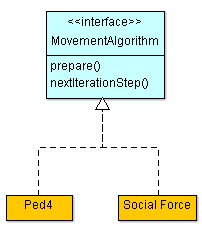
\includegraphics[scale=0.75]{./img/move_algos.png}
        \caption{Interfejs \emph{MovementAlgorithm} i jego realizacje}
        \label{fig:movealgo}
    \end{figure}

        \subsection{Social Force}
        \label{sec:social-force-impl}

Poniżej przedstawiono pseudokody metody odpowiedzialnej za ruch "do przodu" w algorytmie Social Force:

\begin{algorithm}
\caption{Ruch agenta w algorytmie Social Force}
\label{alg1}
\begin{algorithmic}
\Procedure{nextIterationStep}{}
    \If{brak możliwości ruchu}
        \State obróć agenta
        \Comment{umożliwia przeszukanie nowych obszarów}
    \Else
        \State cel $\gets$ wyznacz\_pole\_o\_najwiekszym\_potencjale()
        \State przesuń agenta na docelową płytkę
        \State odzwierciedl kierunek wykonanego ruchu poprzez zmianę zwrotu agenta
    \EndIf
\EndProcedure
\newline
\Function{wyznacz\_pole\_o\_najwiekszym\_potencjale}{}
    \State dostepne\_pola $\gets$ wyznacz\_dostepne\_pola()
    \ForAll{dostępne pole}
        \State uwzględnij wartość pola potencjału innych ludzi i odległość od celu
    \EndFor
    \If{agent jest zmęczony}
        \State zwiększ dodatkowo potencjał dostępnego pola najbliżej celu
    \EndIf
    \State pozostaw pola o najwyższym potencjale \\
    \Return{pole leżące najbliżej celu}
\EndFunction
\newline
\Function{wyznacz\_dostepne\_pola}{}
    \State pola\_agenta $\gets$ pola w sąsiedztwie von Neumanna leżące w półkolu wyznaczonym przez kierunek ruchu agenta
    \State pola\_celu $\gets$ pola w sąsiedztwie von Neumanna leżące w półkolu wyznaczonym przez kierunek do celu \\
    \Return{pola\_agenta AND pola\_celu}
    \Comment{część wspólna zbiorów}
\EndFunction
\end{algorithmic}
\end{algorithm}


\indent Funkcja wyznaczająca dostępne pola ogranicza możliwoś ruchu tak, aby agent albo dalej przemieszczał się po dotychczasowej trajektorii, albo skręcił w stronę celu. \\
\indent Potencjał pola obliczany jest na podstawie siły oddziaływania innych ludzi (ujemna składowa) oraz odległości pola od celu (dodatnia składowa). W przypadku, gdy agent już dość długo zmierza do celu (tzn. przebyta przez niego droga znacząco przekracza minimalną drogę konieczną do osiągnięcia celu), lecz nie może go osiągnąć, przestaje zwracać taką uwagę na innych agentów – efekt ten został osiągnięty przez dodatkowe zwiększenie potencjału dostępnej płytki leżącej najbliżej celu. \\
\indent W przypadku, gdy brak jest dostępnych płytek, agent obraca się odrobinę w miejscu, by w następnym kroku zyskać nowe możliwości ruchu (ze względu na zmianę zbioru dostępnych płytek).

\newpage
    \section{Symulacja i analiza wyników}
    \label{sec:sim}

    % TODO Stworzyć i opisać przykładowy problem (albo dwa), takie jak mały sklep, czy duże centrum.
    % TODO Zasymulawać przykładowy problem i zebrać dane.

        \subsection{Kalibracja i walidacja parametrów symulacji}
        \label{sec:p}

        % TODO Opisać metody kalibracji i walidacji parametrów symulacji.

        \subsection{Uzyskane wyniki ilościowe i jakościowe}
        \label{sec:results}

        % TODO Opisać otrzymane wyniki, przedstawić statystyki zachowań,
        % TODO czasów spędzonych w centrum handlowym itp.

        \subsection{Wyniki symulacji a rzeczywistość}
        \label{sec:sim-vs-reality}

        % TODO Napisać dokładne porównanie z rzeczywistymi danymi.

\newpage
    \begin{thebibliography}{9}
        \label{sec:refs}

        \bibitem[Wąs, Gudowski, Matuszyk 2006]{refs:social-distances-1} - Social Distances Model of Pedestrian Dynamics
        \bibitem[Karakayali 2009]{refs:social-distances-2} - Social Distance and affective orientation
        \bibitem[Blue, Adler 2000]{refs:4-way-movement} - Modelling Four Directional Pedestriam Movements
        \bibitem[Blue, Adler 2001]{refs:cellular-movement} - Cellular automata microsimulation for modeling bi-directional pedestrian walkways
        \bibitem[Bitgood, Dukes 2005]{refs:movement-economy} - Economy of Movement and Pedestrian Choice Point Behavior in Shopping Malls
        \bibitem[Borgers, Timmermans 1986]{refs:route-choice-1} - A Model of Pedestrian Route Choice and Demand for Retail Facilities within Inner-City Shopping Areas
        \bibitem[Borgers, Timmermans 1986]{refs:route-choice-2} - City centre entry points, store location, patterns and pedestrian route choice behaviour: a microlevel simulation model
        \bibitem[Borgers, Timmermans 2005]{refs:pedestrian-behaviour-1} - Modelling pedestrian behaviour in downtown shopping areas
        \bibitem[Kitazawa, Batty 2004]{refs:pedestrian-behaviour-2} - Pedestrian Behaviour Modelling - An Application to Retail Movements using a Genetic Algorithm
        \bibitem[Zacharias 2000]{refs:real-data-1} - Shopping behavior at Alexis-Nihon Plaza in Montreal
        \bibitem[Rauh, Schenk, Schrődl 2011]{refs:real-data-2} - The Simulated consumer - an agent-based approach to shopping behaviour
        \bibitem[Helbing 1992]{refs:fluid-dynamics} - A Fluid Dynamic Model for the Movement of Pedestrians
    \end{thebibliography}
\end{document}
